\chapter{基于双向跨模态实体重构的神经机器翻译}

% 改进:
%    删去的:解码器、短语重构、目标端重构
%    增加的:文本->重构,句子级语义融合
%上一章提出了一种基于明确的图文实体替换的文本重构方法,该方法能够利用图片中视觉目标所携带的信息提升实体词的翻译准确率。虽然为整体的翻译准确率带来了一定的提升,但其一方面采用的是图片到文本单向的重构方法,相关研究表明由文本生成图像的过程也能够提升神经机器翻译的翻译质量;另一方面,原文到原文的生成过程将大量的训练资源浪费在将源端的单词复制到目标端,仅做到了将文本上下文信息融合到视觉目标对应的单词中,却难以将视觉信息融合到文本上下文中。
上一章提出了一种基于显式图文实体替换方案的文本重构方法,该方法能够利用图片中视觉目标所携带的信息提升实体词的翻译准确率。
为了更精确地将重构过程作用到文本实体和视觉实体的表示优化中,并增强视觉实体信息与文本上下文之间的语义融合。本章提出了一种基于双向跨模态实体重构的神经机器翻译方法,该方法在实体重构的基础上增加了基于隐式跨模态信息融合方法的文本非实体重构。
%虽然整体的翻译准确率有一定的提升,但其一方面仅采用了图片到文本单向的重构方法,另一方面,原文到原文的生成过程将大量的训练过程浪费在将源端的单词复制到目标端,难以将视觉信息融合到文本上下文中。
%虽然有效,但模型也在学习复制过程,抛弃了图片信息与文本信息的相互融合。
%为解决以上问题,本章提出了一种基于双向跨模态实体重构的神经机器翻译方法,并在训练中增加了将图片中视觉目标信息与文本上下文融合的任务。
所提方法分为视觉目标到实体词的文本实体重构,实体词到视觉目标的视觉实体重构,以及文本上下文与视觉目标组合序列到非实体词的文本非实体重构三个子任务。通过多任务学习将这三个重构任务与翻译任务结合,达到更加充分地利用图片视觉信息的目的,从而提升神经机器翻译模型的翻译质量。
% 实验结果
实验结果展示了所提方法在英德、英法和英捷三个翻译任务上进一步提升翻译质量的能力,在进一步的分析中展示了双向实体重构与文本非实体重构方法组合的有效性。
\section{引言}
%第一部分应该讲一些能够引入sec3不足的方面,即如何更充分的利用视觉信息
%可以从预训练模型的角度去分析仅采用一种task的方式的不足
%本章可以强调多任务的“多”,上一章更应该是双任务
传统的融合图片信息的神经机器翻译方法采取将图片作为额外输入的方式,从而使翻译模型在编码或解码阶段尽可能地利用其所携带的视觉信息。然而这类方法很难达到理想的效果,图片作为外源信息难以被直接利用。相比之下,采用多任务学习的方式将外源信息融合到神经机器翻译中成为一种可行的方案\cite{49_wang-zhang-2022-addressing,50_kang_zong_2022}。


%第二部分从上一章做了哪些具体内容,详细分析其不足,例如为何重构文本存在资源浪费,为何只有文本上下文到视觉目标的融合。
上一章提出的跨模态文本重构方法采用了文本重构任务,尝试在跨模态编码和文本解码生成两个阶段将图片中的视觉目标信息融合到词的表示中,并为模型的翻译质量带来了提升。但该方法仍存在着一定的不足和需要改进的地方:一是所采用的重构方案是单向的,仅考虑了图片到文本方向,文献\cite{37_elliott-kadar-2017-imagination}表明文本到图像的生成同样可以提升模型的翻译质量,因此存在未充分利用视觉信息的可能;二是原文到原文的生成训练,很容易使模型的编码-解码过程收敛为“复制-粘贴”过程,这种极端情况下除了视觉目标对应位置可以从图片以及上下文中获取信息用于生成目标单词,其它词在编码和解码过程中难以融合信息,只是将源语言的词复制并粘贴到目标端的对应位置,使整个重构模型的训练流程大量地浪费在这种“复制-粘贴”过程中。
尽管模型的实际表现并未如此不堪,但以上的分析也说明了方法存在的改进空间。

%如何解决上面的不足:双向重构(文到图的重构会带来哪些作用),文本非实体重构(为何将视觉信息融合到文本中有效果)(这两个问题需要在实验中体现)
为了解决以上问题,本章提出一种跨模态实体重构(cross-modal entity reconstruction,CER)方法用于帮助神经机器翻译提升译文的质量。该方法为了更加充分地将图片中的视觉目标信息融合到实体词的表示中,采取了图片与文本两个模态之间的双向重构策略,实现显式的跨模态信息融合。并且为了进一步提升图片信息的作用,将图片信息与文本上下文信息融合,采用了非实体的重构策略,实现隐式的跨模态信息融合。将显式方法与隐式方法融合到同一个模型中,实现对翻译模型的更进一步的增强。
具体地,CER方法分为三个子任务:
文本实体重构任务延续了上一章文本重构任务利用视觉目标与文本上下文实现重构的策略,区别在于文本实体重构任务省去了非实体词的生成过程,即只重构文本中的实体词;
视觉实体重构任务负责从文本上下文与文本实体中所提供的文本模态信息重构视觉目标实体,区别于重构完整图片的方案,视觉实体重构以更细粒度更精确的方式进行文本到图像的生成任务;
文本非实体重构任务采用部分文本上下文信息与视觉实体的组合,重构文本上下文中非实体词的部分,这样能够使图片中的视觉目标信息作用到文本的表示学习过程中,区别于上一章的文本重构方法也重构了文本非实体,本章在进行文本非实体重构时需要将源端的对应非实体信息通过掩码的方式去除,确保重构过程不是简单地从源端复制信息。
CER-NMT是结合了跨模态实体重构和非实体重构的神经机器翻译方法。在CER-NMT中,翻译任务作为主任务与CER方法的三个子任务通过多任务训练的方式相结合,从而实现对模型翻译准确率的提升。

%贡献:实体级图片重构,显式方法与隐式方法的融合,
本章主要贡献如下:

(1)本章提出了一种基于双向跨模态实体重构的神经机器翻译方法。在文本重构任务的基础上,增加了视觉实体重构和文本非实体重构两个任务,使图片中的视觉目标信息能够更充分的分别融合到句子中的文本实体与文本上下文中,最终通过多任务学习的方式增强翻译模型的表示能力,达到提升译文质量的目的。
%使得在文本的表示学习过程中图片中的视觉目标信息能够更充分地融合到

(2)本章所提方法结合了显式与隐式两种跨模态信息融合方法。文本实体重构与视觉实体重构均采用了显式跨模态实体信息融合方法,即图片信息具有明确的作用目标。文本非实体重构采用了视觉信息与文本上下文信息,因为非实体词与视觉目标没有直接的对应关系,因此视觉信息的作用目标不明确,属于隐式跨模态信息融合方法。通过结合两类方法实现对翻译模型的进一步的增强。

(3)本章所提方法使模型的翻译质量得到了进一步的提升。在对实验结果的分析中发现,CER方法能够提升模型的翻译忠实度,使翻译过程更忠于原文所提供的实体词的信息。在更进一步针对词频的翻译准确率的统计中发现,实体重构方法能够有效提升主要分布于低频词的实体词的翻译准确率,非实体重构方法对非实体词也有一定的相似效果。
% 应该强调一下多粒度跨模态信息融合方法,一个明确的粒度是实体机双向融合,另一个是句子级跨模态信息融合
\section{相关工作}
本章主要关注在图片增强式的神经机器翻译模型中,使用多种图文重构任务来增强纯文本翻译质量。相关工作可以分为以下两类:

{\sffamily (1)图片重构}

图片不仅可以作为信息提供者为模型在翻译过程中提供需要补充的信息,也可以作为语义的参考媒介,帮助模型在训练过程中增强语义的表示能力。相对于句子到图像的生成问题,早期研究主要解决跨模态的语义对齐的问题。\tcite{nakayama2017zero}将源语言句子、目标语言句子以及图片映射到一个统一的表示空间,在解码的过程中,解码器可以将来自不同模态的编码表示解码到目标语言句子。\tcite{chen2019from}提到图片相对于句子包含了更多与句子不相关的语义,难以作为句子级语义信息的媒介,因此提出了将图片作为词级翻译的媒介,并将词级翻译的结果应用到句子级的零资源翻译中。

以图片信息作为语义媒介的研究可以视为图片重构的先驱研究,因为这种语义的映射方式与利用句子生成图片的本质是相同的。然而,图片包含着比句子更完整且更丰富的信息。在面向翻译任务时,图片中大部分信息相对于待翻译的源语言句子实际上是冗余的。因此,在进行图片重构时,文本信息只能重构图片中的部分信息。\tcite{elliott2017imagination}为纯文本神经机器翻译设计了“想象力”机制。区别于直接生成与图片相对应的图片特征,该机制采用余弦相似度作为语义距离的衡量方法,拉近文本表示与图片特征的语义相似度。\tcite{zhou2018visual}在“想象力”机制的基础上增加了图像特征到文本的注意力机制,生成的上下文向量能够关注到与图片内容相关的源端词,通过初始化的方式将视觉信息提供给解码器。\tcite{long2021generative}采用生成对抗网络(generative adversarial networks,GAN)强化“想象力”机制。该方法使用注意力机制将源语言的词级表示用于生成与图片特征一致的向量表示,在解码阶段同样会使用到“想象”得到的特征向量,从而实现在编码阶段生成图片,在解码阶段利用生成的图片信息。

区别于上述这些方法利用句子级别的语义信息生成图片,本章所采用的视觉实体重构方法主要针对视觉目标的语义重构。一方面,图片中包含着相对于句子更多冗余的信息,这些冗余信息难以从句子的语义信息重构出来的;另一方面,视觉目标所包含的语义信息更集中,提取视觉目标的过程已经过滤掉大量的背景信息,使词到视觉目标的实体级重构更容易。


{\sffamily (2)视觉语言预训练方法}

图片信息与文本信息相融合的方法广泛应用于基于视觉语言预训练模型(vision-language pre-trained model)的自然语言理解任务(natural language understanding,NLU)中。
%文献【】采用了句子与图片的视觉目标序列的组合输入方式,在BERT的初始化参数基础上,通过对文本序列和视觉目标序列
\tcite{li2019visualbert,li2020unicodervl,su2020vlbert,chen2020uniter}采用了BERT\pcite{devlin2019bert}与Faster R-CNN\pcite{ren2015faster}的组合方式,首先将输入图片输入到Faster R-CNN中提取多个视觉目标特征,然后将这些视觉目标特征当作图片序列同文本序列一起输入到以BERT为初始化参数的编码器中,最后通过多种预训练任务实现跨模态信息的融合。这其中常见的预训练任务有:(1)掩码语言模型(masked language modeling),该任务能够以文本为上下文,通过视觉目标所提供的视觉信息预测被掩码的单词,该过程能够将视觉信息融合到文本语义中;(2)图文匹配(image-text matching),该任务需要模型判断当前输入的句子和图片的内容是否一致。
\tcite{lu2019vilbert,tan2019lxmert}则采用了双流模型(dual-stream model)的结构,即图片和文本两个模态的序列需要各自编码再交叉编码的方式,试图通过模态内(intra-modality)和模态间(cross-modality)编码的组合方式,加强跨模态信息融合的能力。
\tcite{huang2020pixelbert,kim2021vilt,li2021align}则希望图片在输入到模型时尽可能的保留全部的视觉信息,因此放弃了应用提取视觉目标的方案,将完整的图片或图片特征输入到了模型中。

区别于这些方法通过大量数据驱动的方式实现跨模态信息的融合,本章所提方法在文本非实体重构过程中使用视觉目标明确地替换文本中相对应的名词,而重构过程则是针对非实体词的重构。该过程虽然保留了显式的视觉信息作用方式的同,但在重构过程中使用视觉目标信息与文本上下文信息融合为跨模态上下文信息,在重构非实体词的过程中并非直接利用视觉目标的信息,因此文本非实体重构更满足隐式跨模态信息融合的特点。


% 文本到图片的翻译


% 多任务nlp,最好是翻译

% 预训练模型:文本、多模态


% 应该侧重图片重建相关的方法,大概也就3个工作(imagination,Adversarial reconstruction for Multi-modal Machine Translation,

\section{方法描述}

\subsection{图文实体}
\label{sec:4_entities}
\begin{figure}[!htbp]
    \centering
    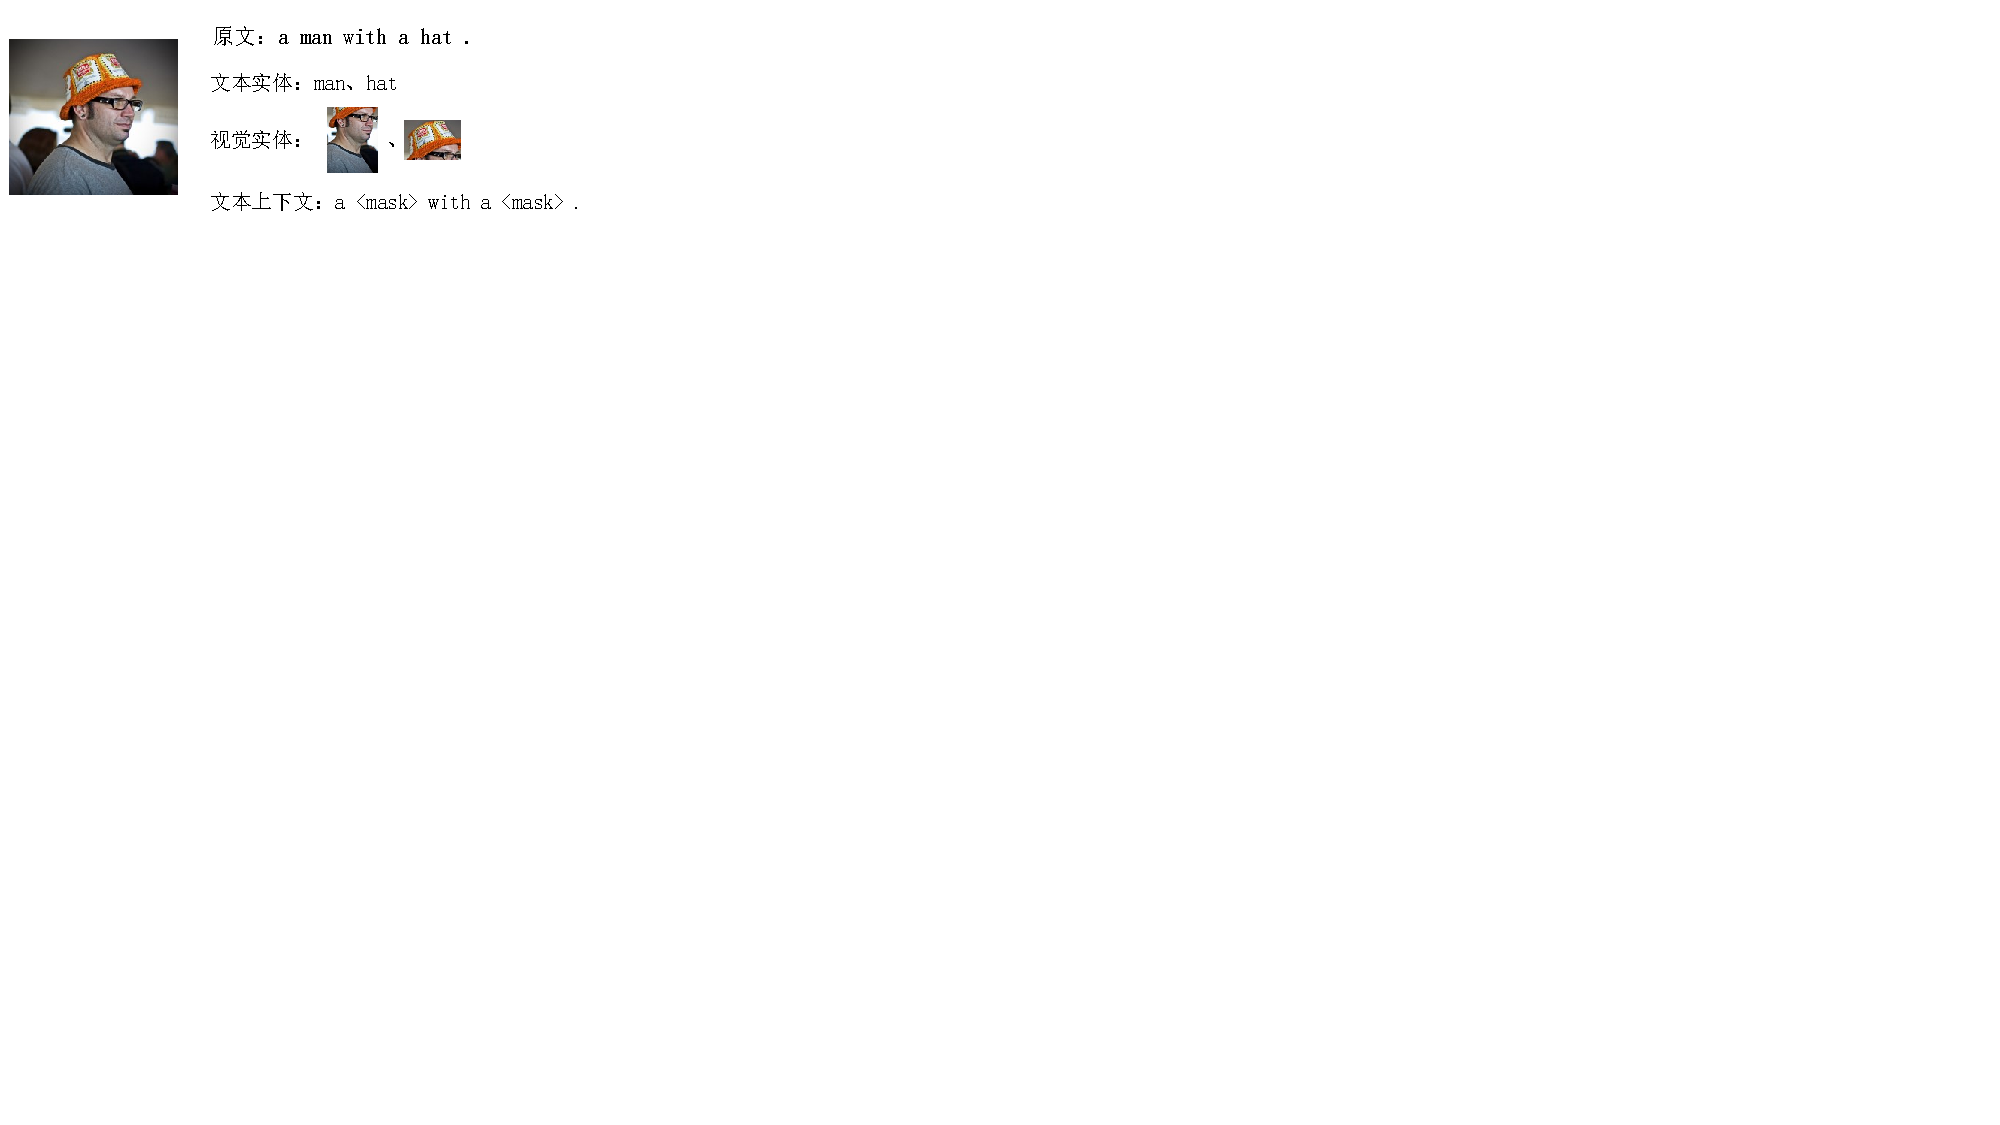
\includegraphics{Img/fig_4_definations.pdf}
    \bicaption{图文实体}{Visual and textual entities}
    \label{fig:4_definations}
\end{figure}
为了更方便地对本章所提CER方法进行介绍,首先需要对CER方法作用到的视觉目标和文本中的作用目标进行恰当的定义:

(1){\sffamily 文本实体:}输入的源语言句子$X=\{x_1,x_2,\cdots,x_N\}$中,$x_i$代表句子中的每个单词,在句子的对应图片中有对应视觉目标的名词$t_a=x_a,t_b=x_b,\cdots$为文本实体(textual entity),$T=\{t_a,t_b,\cdots\}$为它们的集合,可见$T \subseteq X$。如图\ref{fig:4_definations}所示,名词“man”和“hat”在图片中均有与其对应的视觉目标,因此符合文本实体的定义。从该定义同样可知,文本实体与上一章\ref{sec:3_entity_replacement}小节所介绍的词实体本质上是相同的。本章不再将名词短语划为实体范畴进行考虑,只针对名词融合视觉信息。

(2){\sffamily 视觉实体:}文本实体在对应图片$I$中的对应视觉目标$v_a,v_b,\cdots$为视觉实体(visual entity),$V=\{v_a,v_b,\cdots\}$为它们的集合。图\ref{fig:4_definations}中的“男人”和“帽子”分别是文本实体“man”和“hat”在图片中对应的视觉目标,因此是视觉实体。

(3){\sffamily 文本非实体:}在源语言句子中,所有不是文本实体的单词均可称为文本非实体(textual none-entity)。$\tilde{X}=X-T$代表它们的集合、文本上下文或退化文本。例如图\ref{fig:4_definations}中,文本上下文中除了特殊单词“<mask>”均为文本非实体。

%\subsection{跨模态编码}
%\label{sec:4_cross_modal_encoding}
%\begin{figure}[!htbp]
    \centering
    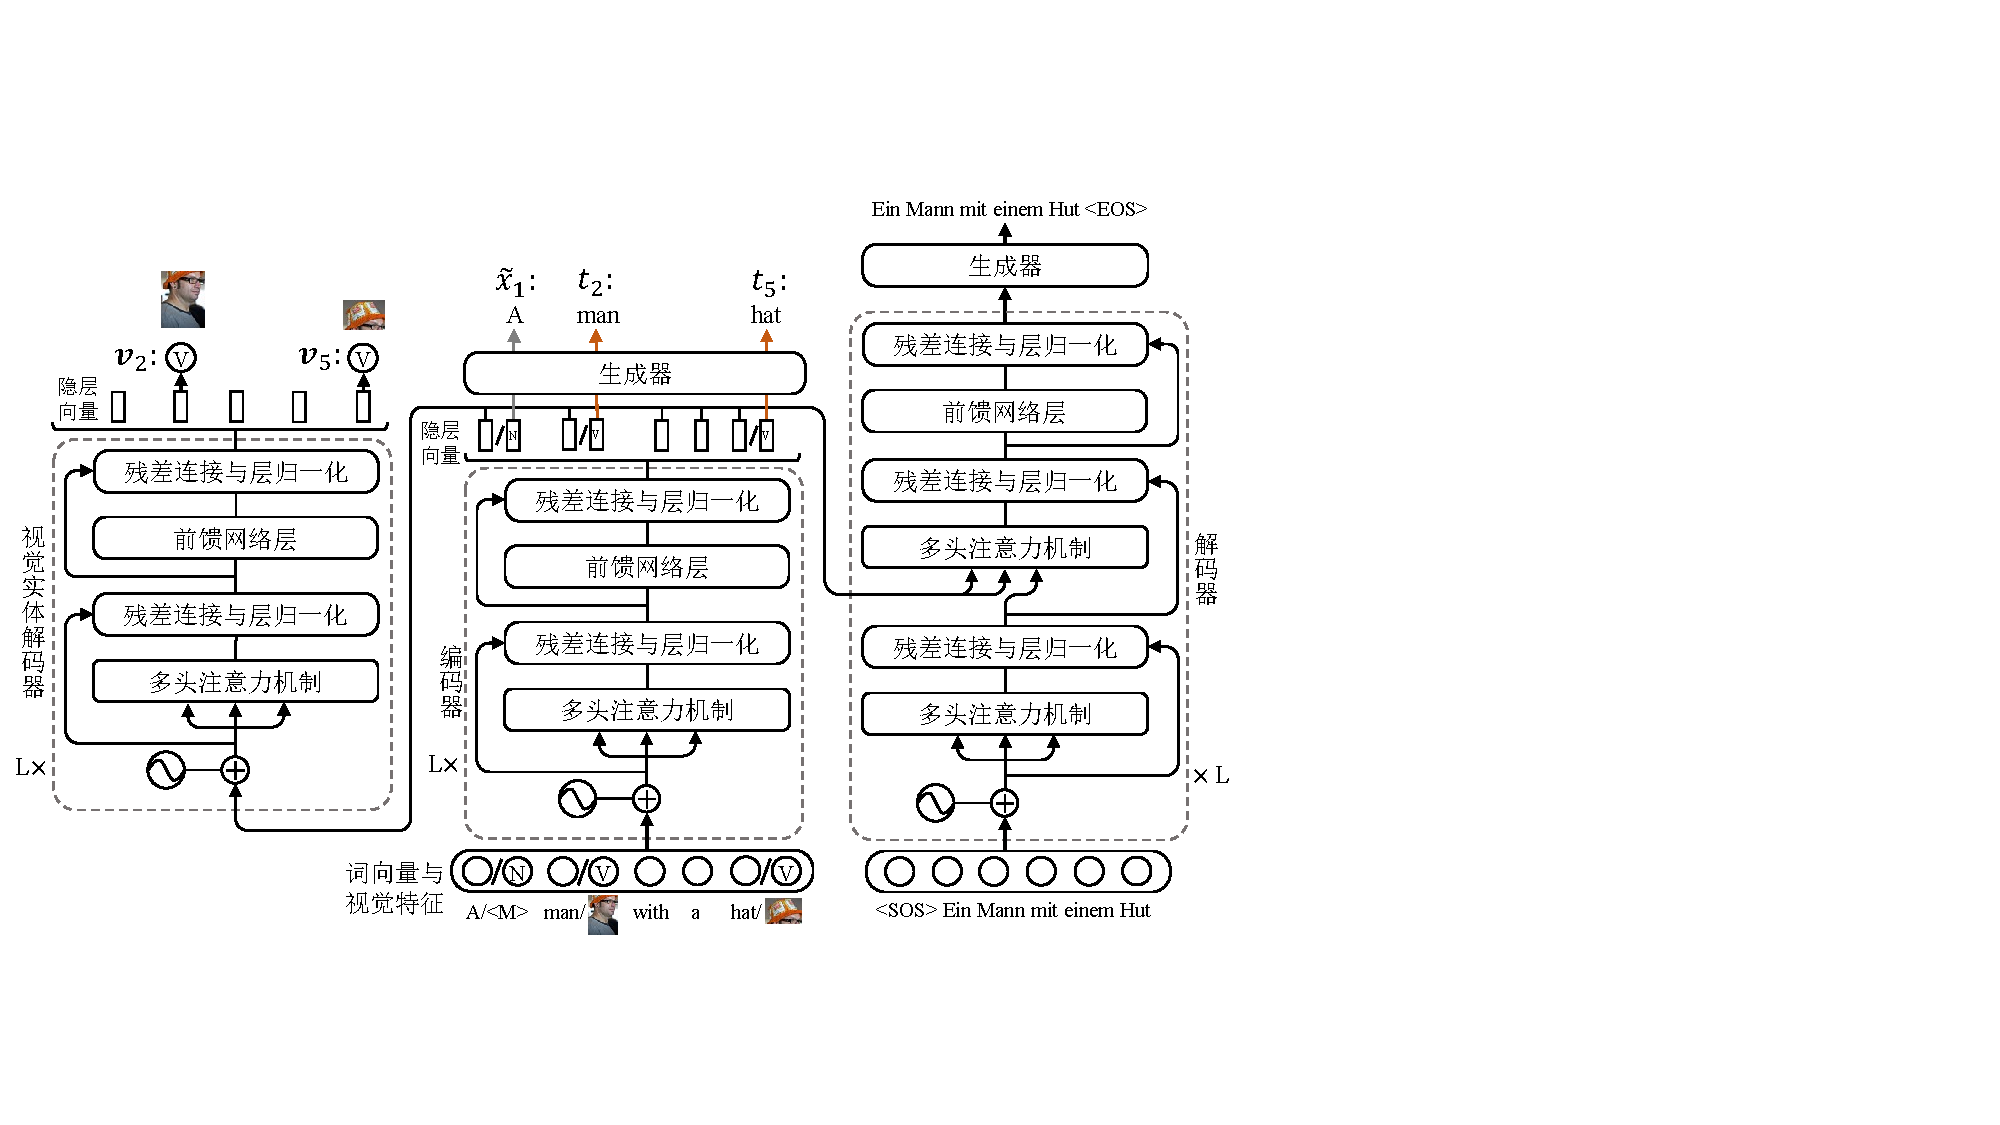
\includegraphics[scale=0.65]{Img/fig_4_model.pdf}
    \bicaption{结合跨模态实体重构方法的神经机器翻译}{NMT model framework combined with CER}
    \label{fig:4_model}
\end{figure}
%图\ref{fig:4_model}展示了CER模型与NMT模型相融合的简化过程,其中包含了视觉实体解码器、跨模态编码器以及翻译解码器三个主要组成部分。其中最核心的跨模态编码器负责在实体重构之前将视觉信息与文本信息编码融合。所编码的信息包含着实体重构主要依赖的三部分:

%\begin{itemize}
%\item
%\begin{figure}[!htbp]
    \centering
    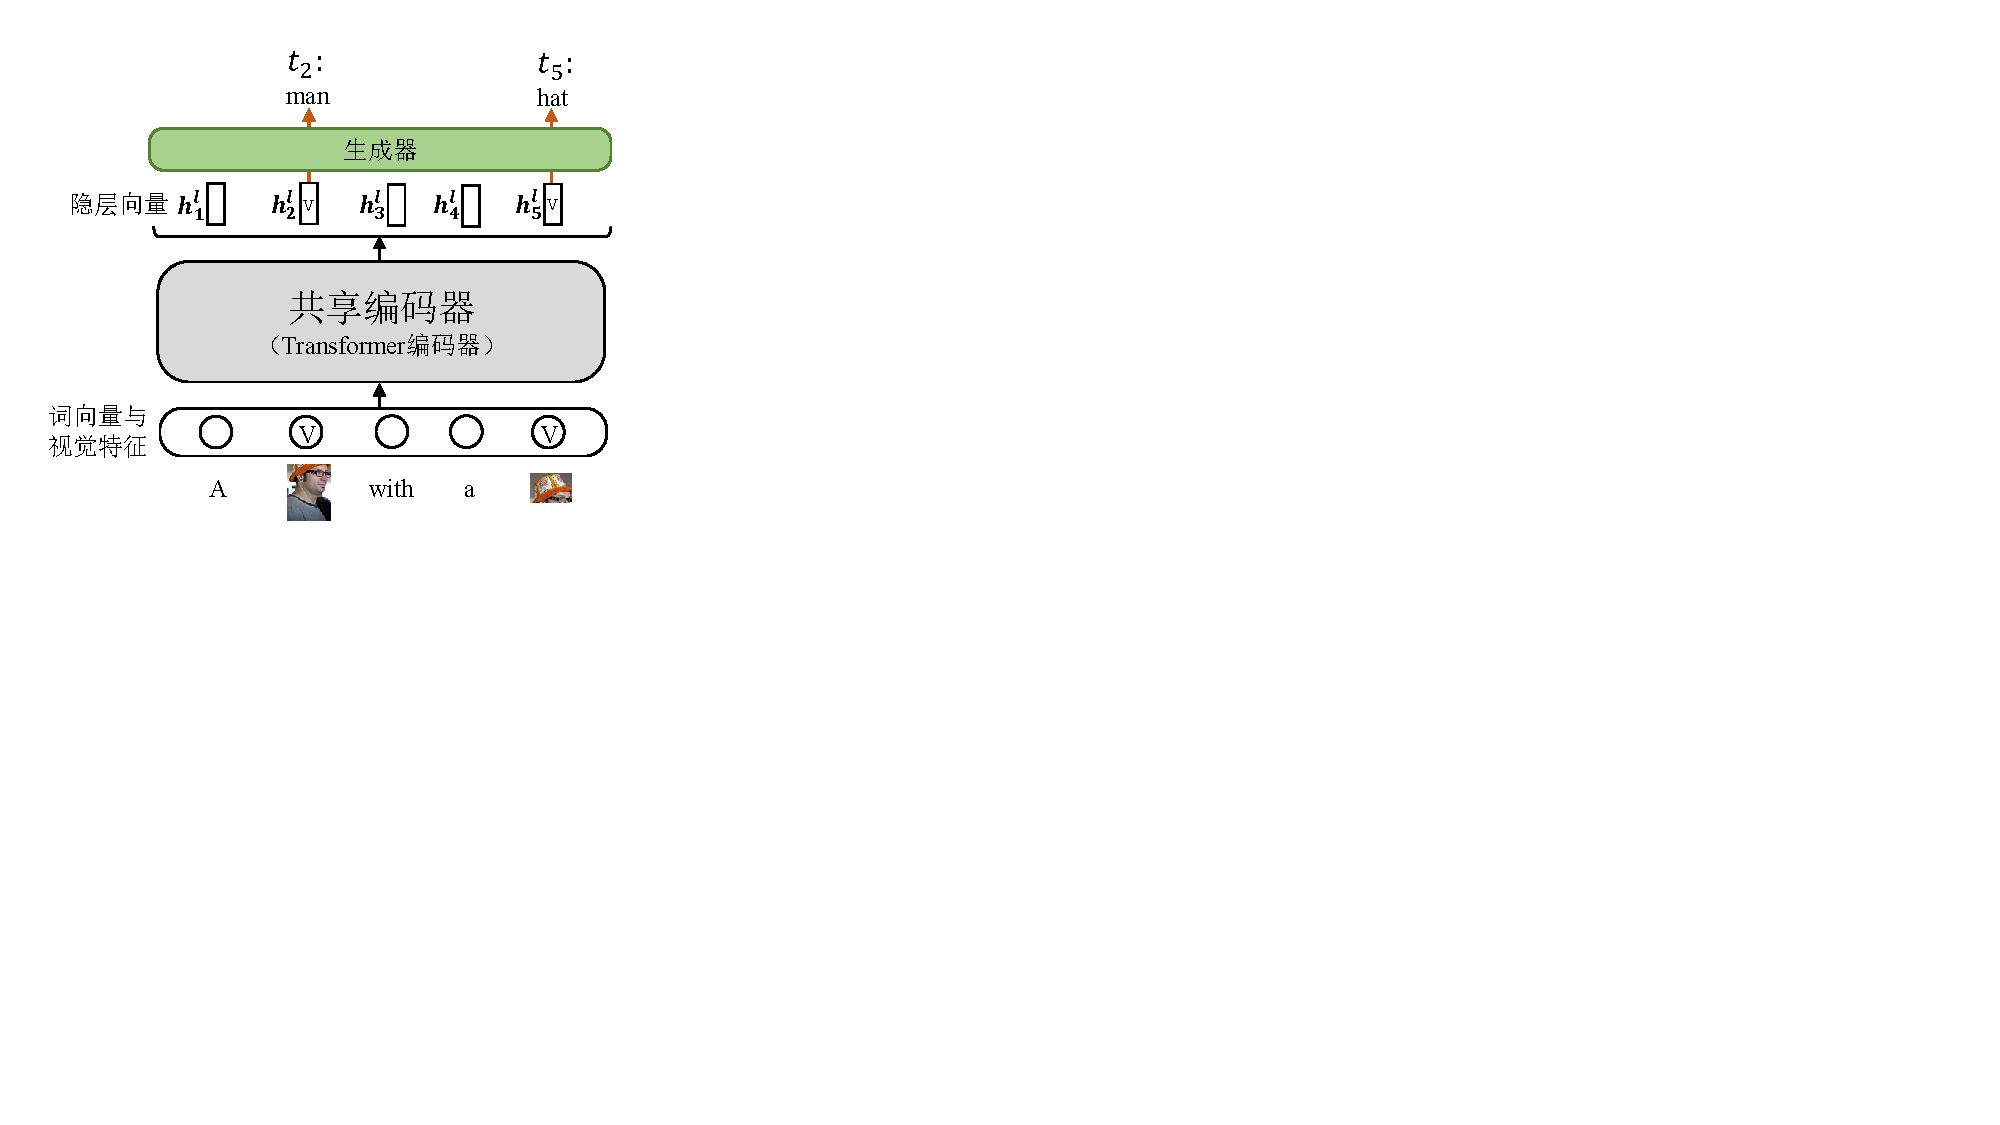
\includegraphics[scale=0.7]{Img/fig_4_ter.pdf}
    \bicaption{文本实体重构}{Textual entity reconstruction}
    \label{fig:4_ter}
\end{figure}
%(1){\sffamily 跨模态实体:}其中实体重构主要依赖于跨模态实体所提供的具体信息。如图【】所示,文本实体$t_1$的重构主要依赖于视觉实体$e_1$,视觉实体$e_1$的重构也主要依赖于文本实体$t_1$。

%\item
%(2){\sffamily 文本上下文:}本文所用文本上下文为经过退化的文本$\tilde{X}$。例如图【】中进行实体重构时,文本上下文为“A <M> with a <M>”,其中“<M>”代表将实体词所对应的位置删除并保留该位置空缺。文本上下文与跨模态实体共同组成文本的完整语义。在进行视觉实体重构时,模型的输入由文本上下文和文本实体共同组成,即原文本$X$。在进行文本实体重构时,模型的输入是文本上下文和视觉实体所组成的多模态混合序列$Z$。在进行文本非实体的重构时,模型的输入同样是多模态混合序列,但是需要将待重构的非实体词利用掩码词“<M>”替换掉,形成$\tilde{Z}$。跨模态实体与文本上下文组合重构实体的方式,既能保证重构实体时具备充足的语义信息,又能充分利用到自注意力机制的特性使实体与文本上下文建立良好的语义关系。

%\item
%(3){\sffamily 实体对齐关系:}为了避免让模型完成较为困难的跨模态实体关系对齐,本文采用直接替换对应位置向量表示的方式。例如图2中重构文本实体$t_1$时,将输入序列中的对应位置直接替换为视觉实体的向量表示${\boldsymbol{e}_1}$。

\subsection{跨模态实体重构}
\label{sec:4_cer}
\begin{figure}[!htbp]
    \centering
    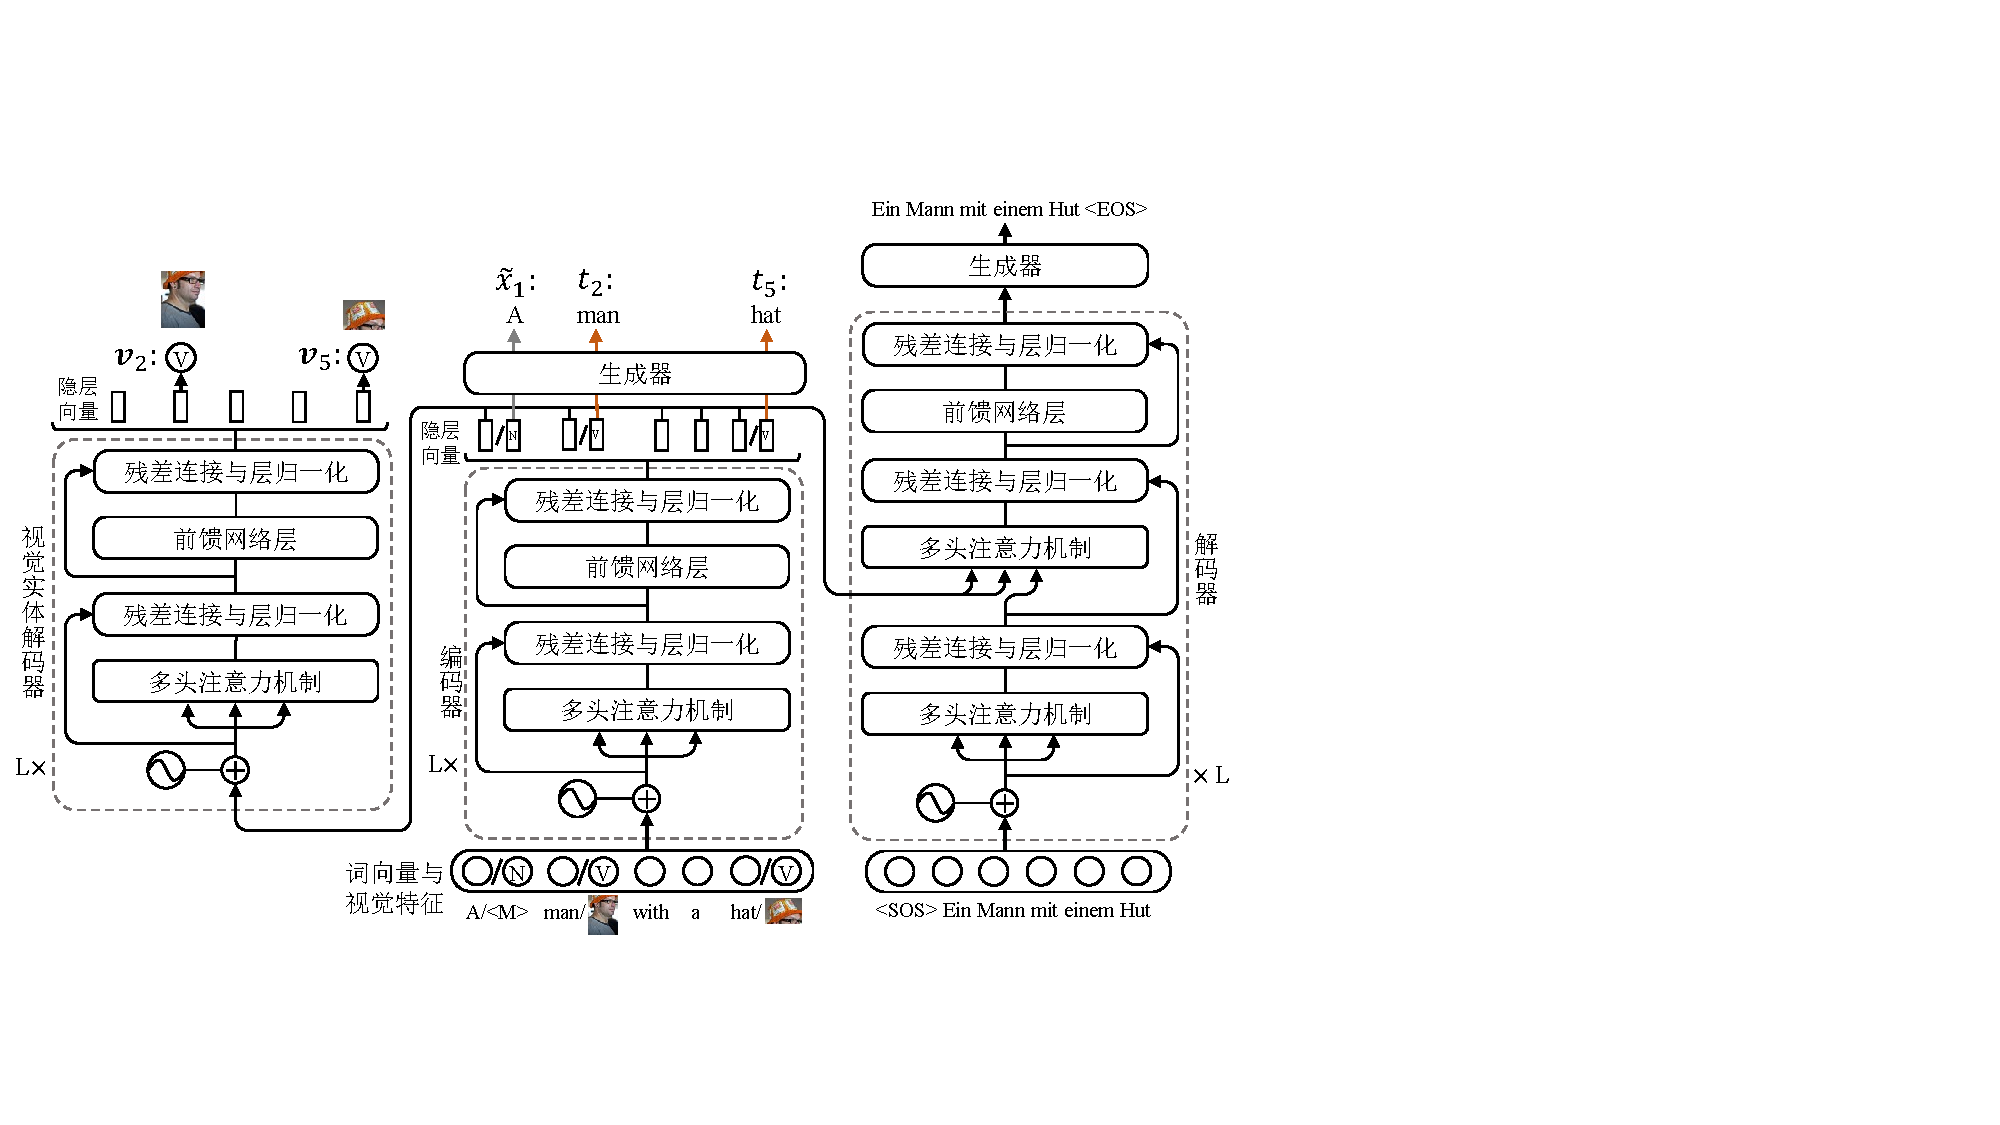
\includegraphics[scale=0.65]{Img/fig_4_model.pdf}
    \bicaption{结合跨模态实体重构方法的神经机器翻译}{NMT model framework combined with CER}
    \label{fig:4_model}
\end{figure}
图\ref{fig:4_model}展示了CER模型与NMT模型相结合的简化结构,其中包含了视觉实体解码器、跨模态编码器以及翻译解码器三个主要组成部分。其中最核心的跨模态编码器负责在实体重构之前将视觉信息与文本信息编码融合。解码器仅用于主任务翻译的目标文本解码。视觉实体解码器负责将跨模态编码器编码后的状态解码到视觉目标所代表的视觉语义空间,而其结构与编码器相同均为$L$层Transformer编码器。为了更详细地介绍CER方法是如何工作的,以及如何与神经机器翻译相结合,本节将CER方法分为:文本实体重构、视觉实体重构以及文本非实体重构三个子任务展开详细的介绍。

{\sffamily (1)文本实体重构}

\begin{figure}[!htbp]
    \centering
    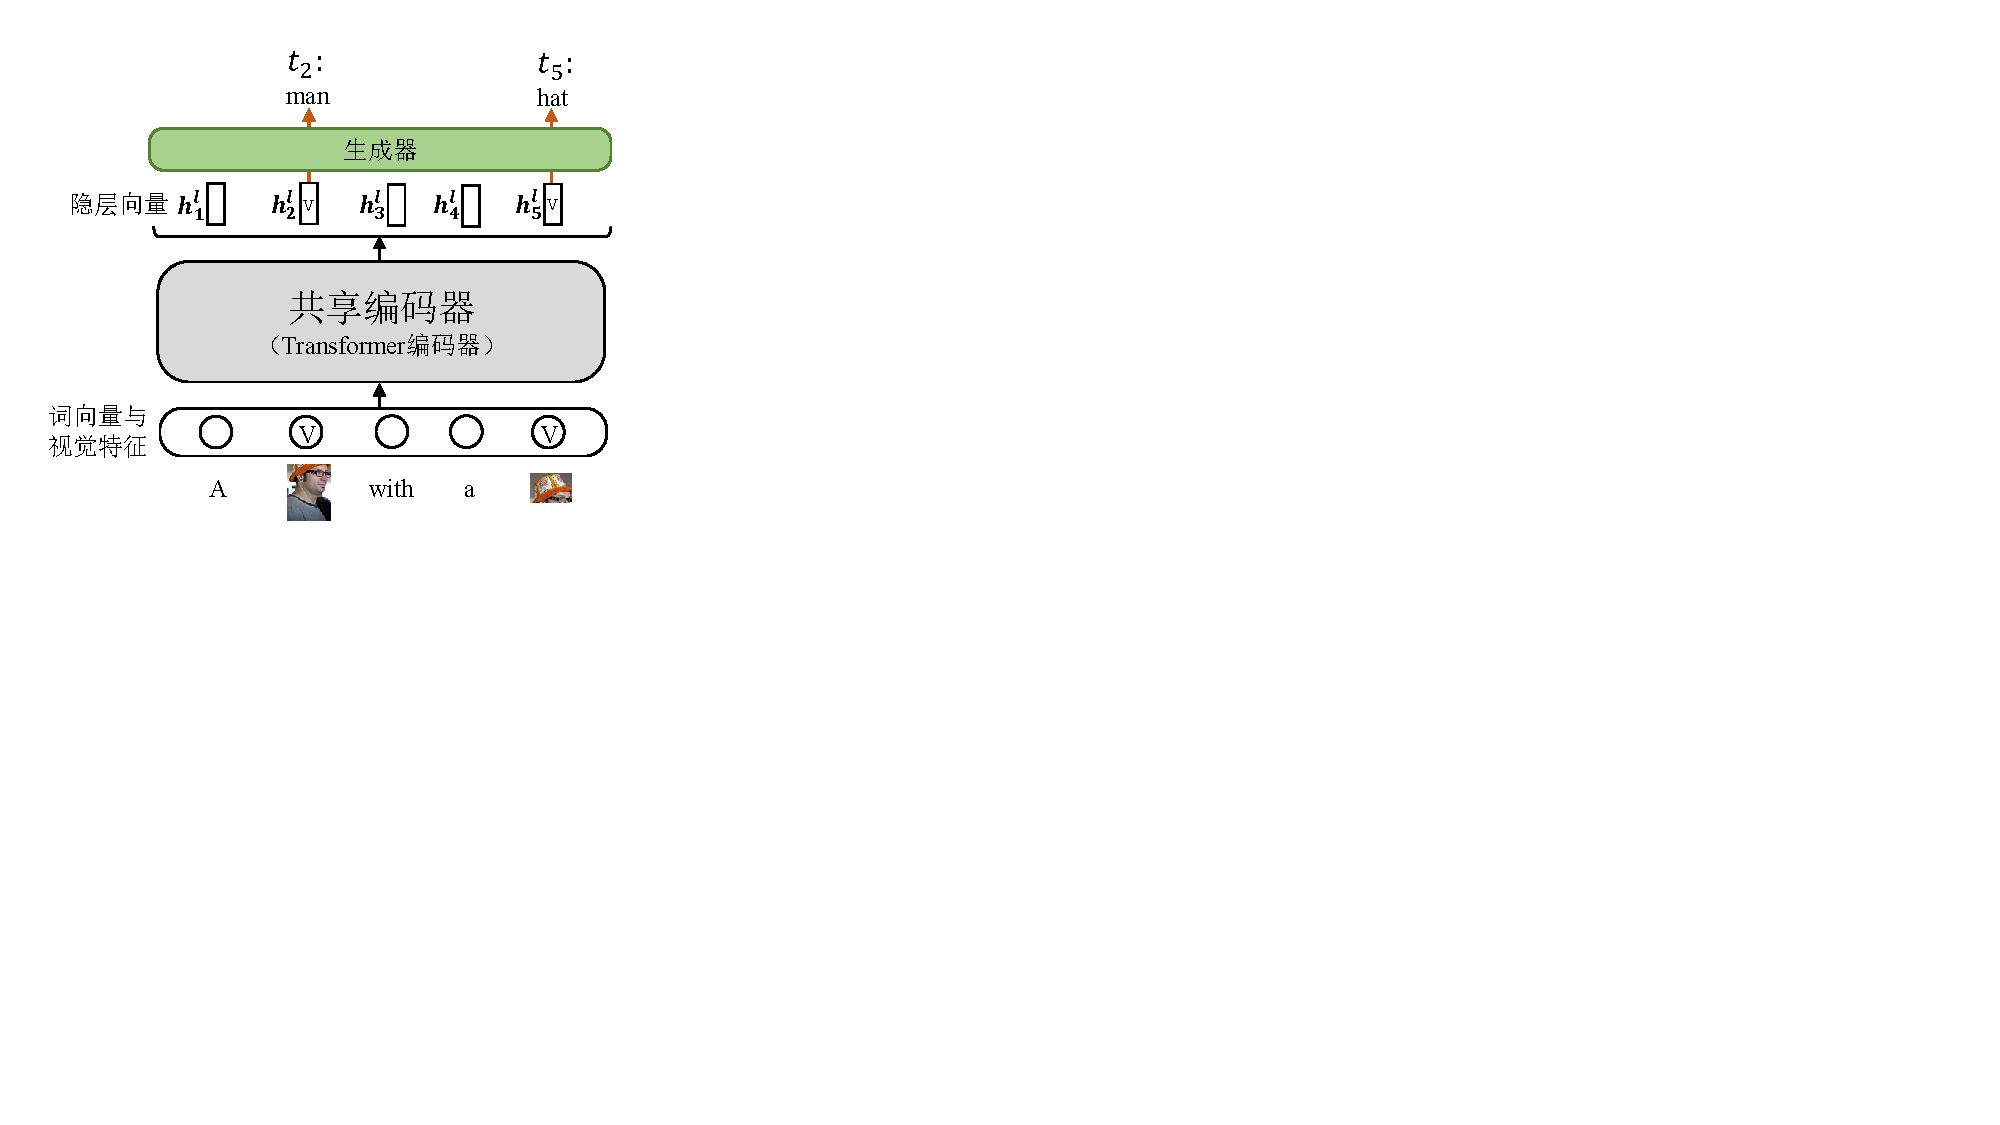
\includegraphics[scale=0.7]{Img/fig_4_ter.pdf}
    \bicaption{文本实体重构}{Textual entity reconstruction}
    \label{fig:4_ter}
\end{figure}
文本实体重构(textual entity reconstruction,TER)与上一章相似,将视觉目标明确地作用到文本实体上。本章仅针对有对应视觉目标的名词采取实体替换,因此文本实体重构的输入为由文本上下文$\tilde{X}$和视觉实体$V$组合成的多模态混合序列:
\begin{equation}
Z={\rm{Combine}} \left( \tilde{X}, V \right)
\end{equation}
如图\ref{fig:4_ter}所示,输入的文本上下文“A <mask> with a <mask>”与视觉实体$\{v_2,v_5\}$组合成多模态混合序列$Z=$“A $v_2$ with a $v_5$”,此时输入到模型中的是三个空心圆代表的词向量和两个标记“V”的圆代表的$v_2$和$v_5$对应的视觉特征。跨模态混合序列经过编码器进行跨模态编码后,得到序列的跨模态表示:
\begin{equation}
\Vector{H_Z^L}={\rm{MultiHead_{enc}^L}} \left( Z, Z, Z \right)
\end{equation}
其中,$\Vector{H_Z^L}=\{\Vector{h_1^l,h_2^l,\cdots,h_N^l}\}$;${\rm{MultiHead_{enc}^L}} \left( \cdot,\cdot,\cdot \right)$代表$L$层采用多头注意力机制的编码器;$\Vector{h_i^l}$中的$l$与$L$相同,代表第$l$层的编码结果。然后依据对应位置的隐层表示生成文本实体,在图\ref{fig:4_ter}中为两个标记“V”的矩形隐层表示${\Vector{h_2^l}}$和${\Vector{h_5^l}}$,该过程需要优化以下损失函数:
\begin{equation}
\mathcal{L}_{\rm{TER}} (\theta, \vartheta) =
    \frac{1}{{\vert}T{\vert}}
    \mathop{\sum}_{x_i \in T}
    {\rm{OH}} \left( x_i \right)
    {\rm log}{\ }{\rm p} \left( Z {\vert} \theta, \vartheta \right)
\end{equation}
\begin{equation}
{\log}{\ }{\rm p} \left( Z {\vert} \theta, \vartheta \right) =
    {\rm{g}} \left( \Vector{h_i^l} \vert \vartheta \right)
\end{equation}
其中${\rm{OH}}\left(x_i\right)$代表$x_i$的独热编码(one-hot,OH)表示,$\theta$代表编码器一端的参数,$\vartheta$为生成器(generator)参数,生成器${\rm{g}}\left(\cdot\right)$将位置$i$处的隐层向量${\Vector{h_i^l}}$映射并得到词表中每个词的预测概率。

{\sffamily (2)视觉实体重构}

\begin{figure}[!htbp]
    \centering
    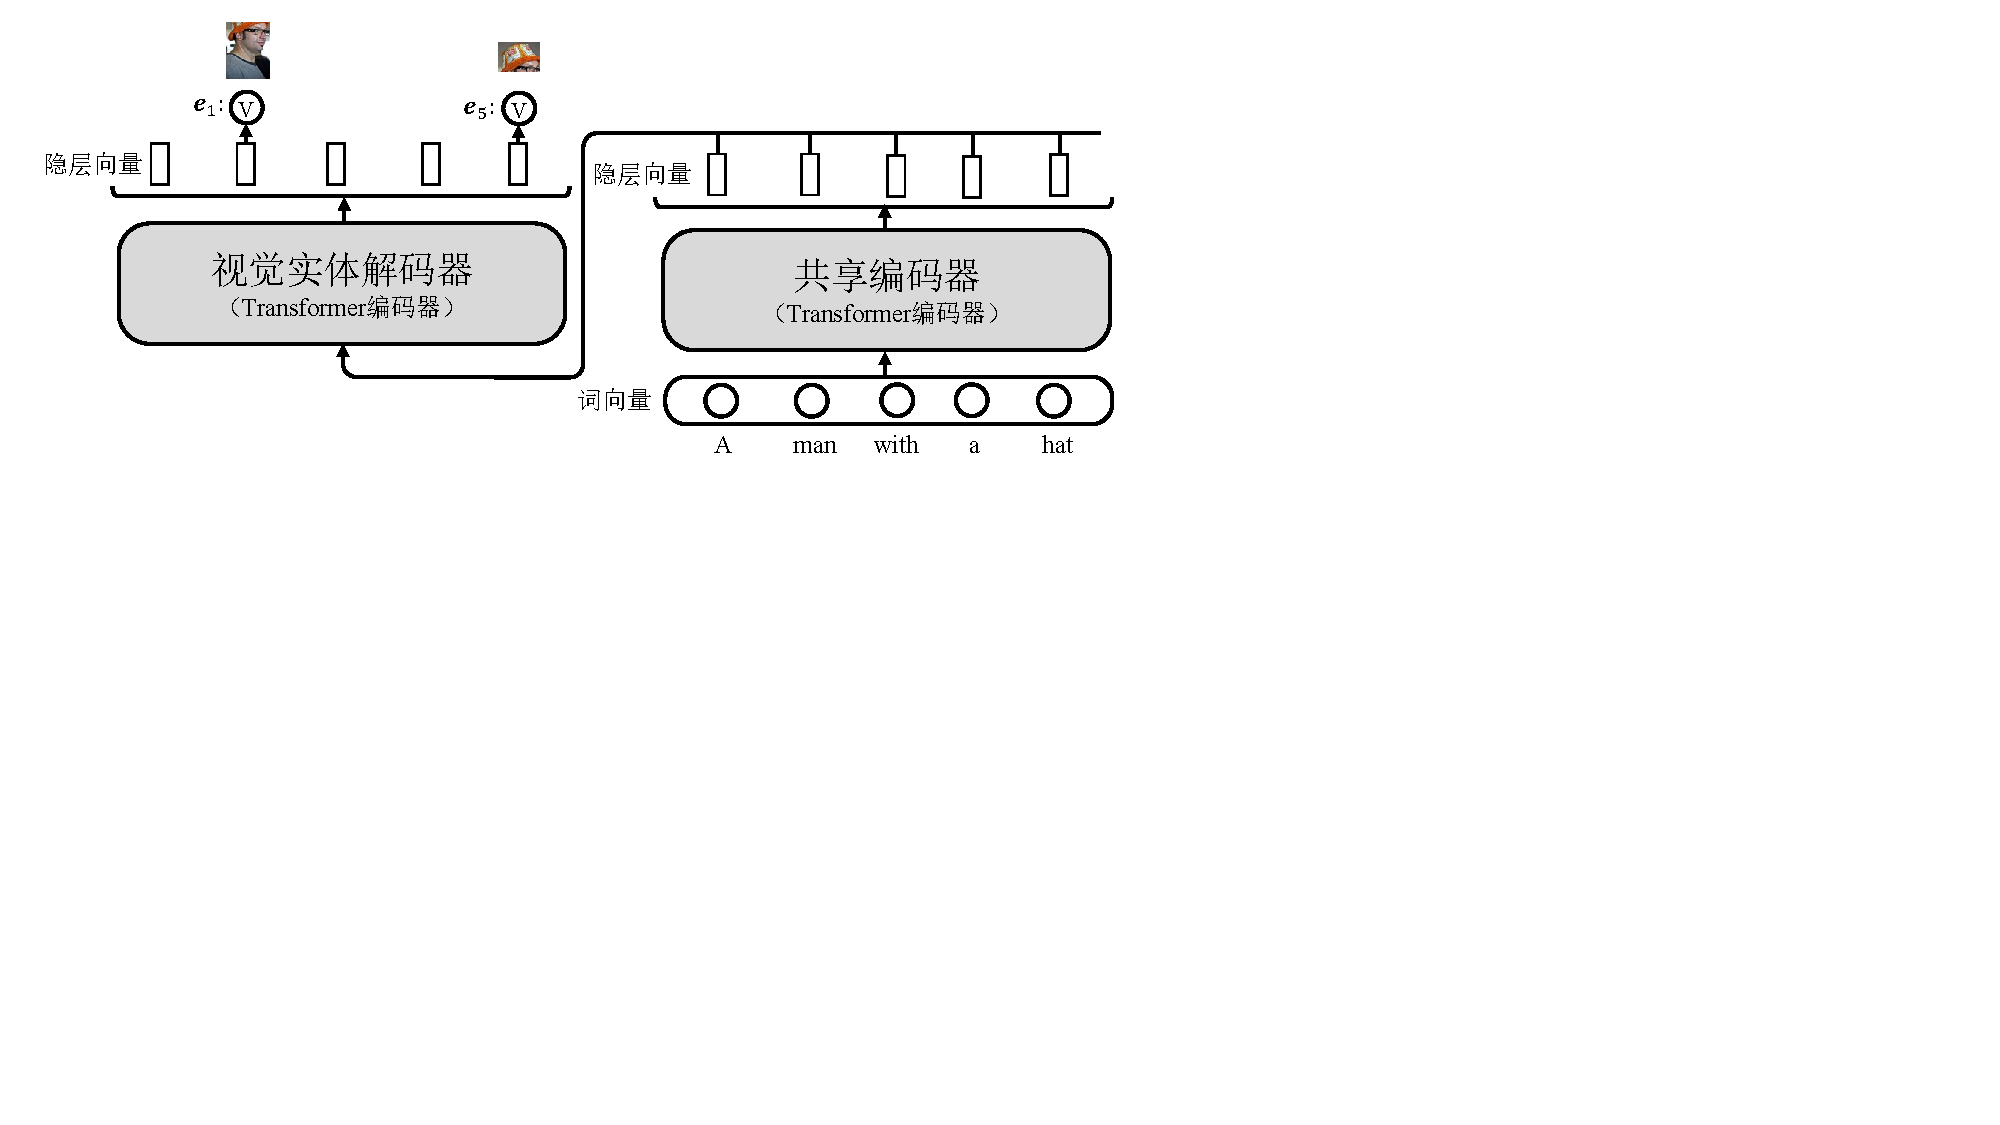
\includegraphics[scale=0.6]{Img/fig_4_ver.pdf}
    \bicaption{视觉实体重构}{Visual entity reconstruction}
    \label{fig:4_ver}
\end{figure}
与文本实体重构不同的是,视觉实体重构(visual entity reconstruction,VER)依赖于来自单一文本模态的$X$。例如图\ref{fig:4_ver}中,“A man with a hat”是重构视觉实体时模型的输入序列,此时图中输入到模型中的是5个空心圆代表的词向量。该句子经过$L$层的编码器进行文本编码,再利用$L$层视觉实体解码器解码出与文本实体$\{t_2,t_5\}$相对应的视觉实体$\{v_2,v_5\}$。由于文本无法完整的描述图片,只是针对图片中的个别属性的描述,由文本直接还原像素级的图片或图片中的视觉实体几乎是不可能的。因此本章仅尝试生成与视觉实体相近的向量表示$\{\Vector{v_2,v_5}\}$。其中,$X$经过如下编码过程:
\begin{equation}
\Vector{H_X^L}={\rm{MultiHead_{enc}^L}}(X, X, X)
\end{equation}
得到编码后的隐层表示$\Vector{H_X^L}=\{\Vector{h_1^l,h_2^l,\cdots,h_N^l}\}$。然后经过如下解码过程:
\begin{equation}
\Vector{H_X^{2L}}={\rm{MultiHead_{dec}^L}}(\Vector{H_X^L, H_X^L, H_X^L})
\end{equation}
得到$\Vector{H_X^{2L}}=\{\Vector{h_1^{2l},h_2^{2l},\cdots,h_N^{2l}}\}$,${\rm MultiHead_{dec}^L}\left( \cdot,\cdot,\cdot \right)$为与${\rm MultiHead_{enc}^L}\left( \cdot,\cdot,\cdot \right)$具有相同结构的视觉实体解码器。然后利用$\Vector{H_X^{2L}}$生成与$\{\Vector{v_a,v_b,\cdots}\}$接近的向量表示,文本采用与\tcite{elliott2017imagination}相近的方式实现该过程:
\begin{equation}
\mathcal{L}_{\rm{VER}}(\theta, \varphi)=
    \frac{1}{{\vert}V{\vert}}
    \mathop{\sum}_{i \neq j}{\max}\{0, \varepsilon - {\rm{cos}}\left( \Vector{h_i^{2l}}, \Vector{v_j} \right) + {\rm{cos}}\left( \Vector{h_i^{2l}}, \Vector{v_i} \right)\}
\end{equation}
%\onecolumn
%\input{docs/model_pic.tex}
%\begin{multicols}{2}
其中$i=a,b,\cdots$为实体在句子中对应的序号;$\varphi$为视觉实体解码器的参数;${\rm{cos}}(\cdot,\cdot)$用于计算向量间的余弦相似度,$\varepsilon$为最小边缘常量。显然,优化$\mathcal{L}_{\rm{VER}}(\theta,\varphi)$能够缩减$\Vector{h_i^{2l}}$与相对应的视觉实体$\Vector{v_i}$之间的余弦距离,增加与其它非对应的视觉实体$\Vector{v_j}$之间的余弦距离。

{\sffamily (3)文本非实体重构}

\begin{figure}[!htbp]
    \centering
    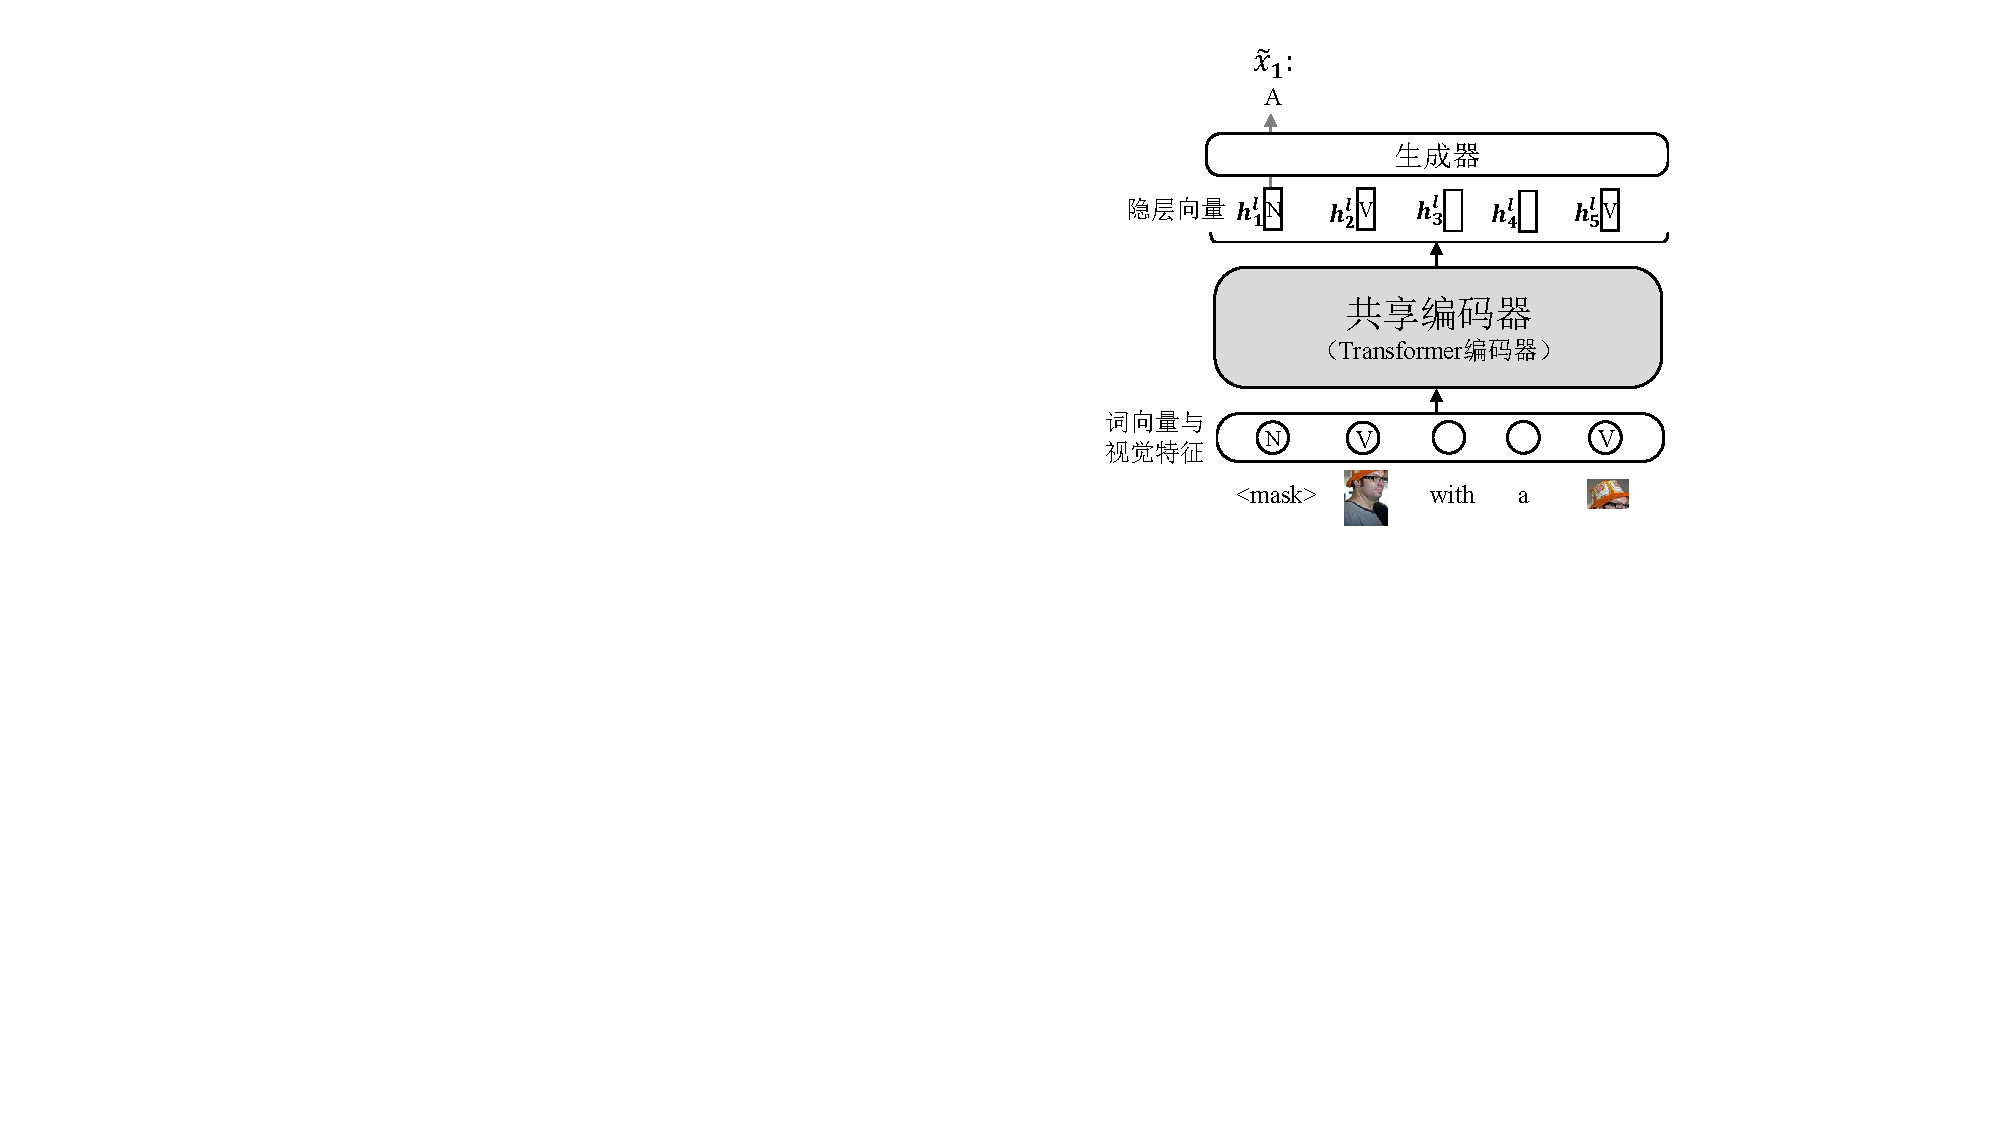
\includegraphics[scale=0.6]{Img/fig_4_tner.pdf}
    \bicaption{文本非实体重构}{Textual none-entity reconstruction}
    \label{fig:4_tner}
\end{figure}
文本非实体重构(textual none-entity reconstruction,TNER)方法与文本实体重构方法相似,区别在于非实体重构的目的是使视觉实体与文本上下文进行充分的句子级语义融合,而实体的重构方法更侧重实体在两个模态之间的实体级语义融合。文本非实体重构时的模型输入同样是文本上下文$\tilde{X}$和视觉实体$V$组合成的跨模态混合序列,但是在$\tilde{X}$中除对实体的位置进行退化还要将待重构的非实体词退化。例如图\ref{fig:4_tner}中,当选择对非实体词“A”进行重构时,模型所输入的跨模态混合序列为$\tilde{Z}=$“<mask> $v_2$ with a $v_5$”,此时输入到模型中的是一个标记“N”的圆形,代表“<mask>”的词向量,以及两个空心圆形所代表的词向量和两个标记“V”的圆形所代表的视觉特征。损失函数如下:
%一个标记``N''的圆形词向量代表``$\langle$M$\rangle$''、两个圆形空心词向量和两个标记``V''的圆形视觉特征. 损失函数如下:
\begin{equation}
\mathcal{L}_{\rm{TNER}}(\theta, \vartheta) =
    \frac{1}{{\vert}\tilde{T}{\vert}}
    \mathop{\sum}_{x_i \in \tilde{T}}
    {\rm{OH}} \left( x_i \right)
    {\rm log}{\ }{\rm p} \left( \tilde{Z} {\vert} \theta, \vartheta \right)
\end{equation}
其中$\tilde{T}$代表待重构的非实体词集,并有$\tilde{T}\subseteq \tilde{X}$。在图\ref{fig:4_tner}中用于预测非实体词“A”的隐层为一个标记“N”的矩形隐层表示$\Vector{h_1^l}$。

本章采用随机选取的方式在句子中选择待重构的非实体词。在执行TNER任务时,每个文本中的非实体词有$30\%$的概率会被选择到。该概率与所采用数据集中实体词占$32.6\%$的比例相近。

{\sffamily (4)CER联合训练}

联合以上所有重构方法的目标函数,可得到本章所提CER方法的联合损失函数为:
\begin{equation}
\mathcal{L}_{\rm{CER}} \left( \theta, \varphi, \vartheta \right) = \alpha \mathcal{L}_{\rm{VER}} \left( \theta, \varphi \right) + \beta \mathcal{L}_{\rm{TER}} \left( \theta, \vartheta \right) + \gamma \mathcal{L}_{\rm{TNER}} \left( \theta, \vartheta \right)
\label{eq:4_combined_cer}
\end{equation}
其中,$\alpha$、$\beta$和$\gamma$为控制三种重构方法训练比例的超参数。值得注意的是,本章没有设置利用纯文本上下文$\tilde{X}$重构文本词的方案。这是因为该方案与一般的预训练方法相似,用于建立纯文本的语言模型。而机器翻译模型的编码端本身就是一个很好的纯文本语言模型,因此不必再设置纯文本的重构方案。

\subsection{与机器翻译相结合}
构建CER模型的目的是辅助翻译模型提升翻译质量。本章采用多任务训练方法将CER方法中的跨模态编码器与神经翻译模型的文本编码器进行参数共享,从而达到对神经机器翻译模型参数优化的目的。翻译任务所要优化的目标函数为:
\begin{equation}
\mathcal{L}_{\rm{NMT}} \left( \theta, \phi \right) =
    -\mathop{\sum}_j^M {\rm log}{\ }{\rm P} \left(y_j \vert y_{<j}, X \vert \theta, \phi \right)
\label{eq:4_nmt}
\end{equation}
其中$Y=\{y_1,y_2,\cdots,y_M\}$为目标语言的文本序列;$\phi$为解码器一端的参数,值得注意的是,在文本实体重构与文本非实体重构中所应用的生成器参数$\vartheta$是$\phi$的一部分,即采用的是同一个生成器。将公式(\ref{eq:4_nmt})与CER模型的损失函数公式(\ref{eq:4_combined_cer})相结合得到联合目标函数为:
\begin{equation}
\mathcal{L} \left( \theta, \phi, \varphi \right) = \omega\mathcal{L}_{\rm{NMT}} \left( \theta, \phi \right) + \left( 1-\omega \right) \mathcal{L}_{\rm{CER}} \left( \theta, \varphi, \vartheta \right)
\end{equation}
其中,用超参数$\omega$调节神经机器翻译与CER方法的训练比例。
\section{实验设置}
\label{sec:4_setup}

\subsection{数据}
\label{sec:4_dataset}


\begin{table}[!htbp]
    \bicaption{Multi30K数据集情况统计}{Statistics about Multi30K dataset.}
    \label{tab:4_datasets}
    \centering
    \footnotesize% fontsize
    \setlength{\tabcolsep}{4pt}% column separation
    \renewcommand{\arraystretch}{1.2}%row space 
    \begin{tabular}{cccccc}
    \hline
      & \multirow{2}*{训练集} & \multirow{2}*{验证集} & \multicolumn{3}{c}{测试集} \\\cline{4-6}
      & & & Test2016 & Test2017 & MSCOCO \\\hline
    图片 & 29000 & 1014 & 1000 & 1000 & 461 \\
    英语 & $\checkmark$ & $\checkmark$ & $\checkmark$ & $\checkmark$ & $\checkmark$ \\
    德语 & $\checkmark$ & $\checkmark$ & $\checkmark$ & $\checkmark$ & $\checkmark$ \\
    法语 & $\checkmark$ & $\checkmark$ & $\checkmark$ & $\checkmark$ & $\checkmark$ \\
    捷克语 & $\checkmark$ & $\checkmark$ & $\checkmark$ &   &   \\
     \hline
    \end{tabular}%
\end{table}%

本章使用融合图片信息的神经机器翻译任务的常用数据集Multi30K\pcite{elliott2016multi30k}测试所提方法的有效性。该数据集每张图片配有一个英文句子和与其对应的德语、法语和捷克语的译文。该数据集的训练集包含29000个平行句对。其验证集和测试集Test2016的大小分别为1014和1000。本章还在常用的测试集Multi30K Test2017以及Ambiguous MSCOCO上进行了测试,其大小分别为1000和461。数据集的具体统计情况如表\ref{tab:4_datasets}所示。值得注意的是,在融合图片信息的神经机器翻译任务中,最常用的是英德翻译数据。其次是英法翻译数据,常用的测试数据为Test2016。而英捷翻译数据仅有很少的应用。

本文采用Moses SMT\pcite{koehn2007moses}工具包对文本数据进行分词和归一化处理。为了防止对视觉实体与文本实体对应关系的破坏,本文并没有采用双字节编码\pcite{sennrich2016neural}(Byte pair encoding,BPE)进行分词处理。在数据的预处理阶段,采用了上一章\ref{sec:3_entity_extraction}节所介绍的方法提取文本实体与视觉实体,并将它们对应起来。最后将视觉实体输入Resnet-50\pcite{he2016deep}提取出2048维的全局图像特征,该特征向量在输入到CER模型的时候会通过一个全连接层映射到与翻译模型词向量相同的维度。

\subsection{模型参数}
\label{sec:4_model_setup}

本章在基于Transformer\pcite{vaswani2017attention}结构的机器翻译模型上进行实验。由于数据集Multi30K的规模相对较小,很容易在Transformer-big或Transformer-base上过拟合,因此本章采用了更小规模的参数设置。本文所设置的参数与\tcite{yin2020novel}基本保持一致,其词嵌入层设置为128维,前馈层为256维。编码器、视觉实体解码器和翻译解码器均为4层,多头自注意力的头数为4。词表采用源语言与目标语言共享的方式,合并后英德翻译的共享词表大小为27226,英法翻译为19393,英捷翻译为29170。利用Adam\pcite{kingma2014adam}优化器优化整个模型参数。本章与\tcite{vaswani2017attention}相同,采用预热和衰减策略来提高学习率,预热步骤为4000,总训练步骤为80000。训练目标中设置平滑标签$\epsilon_{ls}=0.1$。训练时,批数据大小为2000个单词。测试时,采用了搜索空间$b=4$的柱搜索算法。

多任务学习方法的训练方式为随机选择一个任务在当前批数据下对模型进行优化。本文所提CER方法一共包含三个子任务:VER、TER和TNER。这三个任务根据超参数$\alpha$、$\beta$和$\gamma$控制训练的比例。本章将三个子任务的训练比例设置为$\alpha=40\%$、$\beta=40\%$和$\gamma=20\%$。这样保证了CER在训练中将实体级的跨模态信息融合作为主任务,以$80\%$的比例用于跨模态实体重构,$20\%$的比例用于视觉实体与非实体上下文的语义融合。本文将翻译任务设置为主任务,并设置超参数$\omega$为控制翻译任务与CER之间的训练比重。例如当$\omega=0.5$时,NMT与CER的训练比例分别为$50\%$,其中VER、TER和TNER三个子任务的训练比重依据上文调整为$\omega\times\alpha=20\%$、$\omega\times\beta=20\%$和$\omega\times\gamma=10\%$。

%本文所有的模型结果都是在3次随机初始化的条件下训练得到的平均值。最后,通过BLEU4$^{[32]}$和Meteor$^{[33]}$来测试翻译质量,在后面的实验中分别简化为``B''和``M''。


\subsection{对比模型}
\label{sec:4_comparison}

本章将对比方法分为图片信息辅助式和图片信息增强式两类方法。图片信息辅助式方法在训练和测试时均使用额外的图片输入作为上下文信息提升模型的翻译准确率。图片信息增强式则只需要在训练阶段输入图片,通过优化翻译模型的参数来提升模型最终的纯文本翻译质量。本章所提方法属于图片信息增强式方法。图片信息辅助式方法的介绍如下:
%本文将MMT方法分为句子级融合、视觉实体融合以及增强NMT三大类。句子级融合方法主要尝试将视觉信息与整个文本句子进行语义融合。视觉实体融合方法则提预先提取出图片中的视觉目标后再输入到所设计的模型中。增强NMT方法一般在训练中融合视觉信息,而在测试时不需要输入图片。后两类方法中的多数模型在本质上也属于句子级融合方法。各模型简介如下:

\begin{itemize}

\item \textbf{SerialAtt\pcite{libovicky2018input}:}该模型在解码过程中采用了多个交叉注意力串联的形式,每个交叉注意力模块对应了不同的信息来源。在融合图片信息的模型中,两个交叉注意力模块分别用于采集源语言和图片中的信息。

\item \textbf{DelMMT\pcite{ive2019distilling}}模型提出使用推敲网络进行跨模态二次解码。在第二次解码中融合源语言信息、目标语言信息以及视觉信息。

\item \textbf{GAMMT\pcite{liu2021gumbel}:}使用Gumbel-Sigmoid改造注意力机制,帮助翻译模型关注到图片中与文本内容更相关的区域,并排除图片中的噪音。

\item \textbf{GMMT\pcite{yin2020novel}:}该模型视源语言句子与图片中的视觉目标为一个跨模态模态图结构,然后利用设计的基于图的跨模态编码器进行编码,最终解码出目标端句子。
\end{itemize}

图片信息增强式方法的介绍如下:
\begin{itemize}
\item \textbf{Transformer:}基于Transformer的纯文本神经机器翻译模型,其模型配置与\ref{sec:4_model_setup}小节保持一致。
\item \textbf{Imagination\pcite{elliott2017imagination}:}该方法将源语言句子编码后,利用编码后的隐层表示生成与图片的全局特征相近的向量表示,该过程称为“想象力”机制。该方法同样使用了多任务的方式。
\item \textbf{ImagiT\pcite{long2021generative}:}该方法同样采用了“想象力”机制,区别在于ImagiT采用了生成对抗网络,尝试从对原文的编码中“想象”出像素级的图片。
\item \textbf{CTR-NMT:}该模型为本文第3章所设计的方法,采用了词级实体替换方案利用独享解码器重构源语言,是一种图片增强式神经翻译模型。
\end{itemize}
% 实验结果中是否可以展示一下预测词正确的概率,能否与CTR相比下
\section{实验结果}

\subsection{多任务超参数调节}
\label{sec:4_omega}
本章提出的多任务训练方法包含了翻译和CER两个由超参数$\omega$控制训练比例的任务,而CER又包含了TER、VER和TNER三个由$\alpha$、$\beta$和$\gamma$三个超参数控制的子任务。因此如何平衡这些任务的训练比重,对于模型的训练是一个极为重要的问题。本章根据三个子任务的重要程度,将$\alpha$、$\beta$和$\gamma$三个超参数的比例固定为$2:2:1$,然后通过调节超参数$\omega$寻找翻译和CER两个任务之间合适的训练比例。本节依据CER-NMT在英德翻译、英法翻译以及英捷翻译验证集的BLEU值结果选取一个合适的$\omega$值。

%\begin{figure}[!htbp]
%    \centering
%    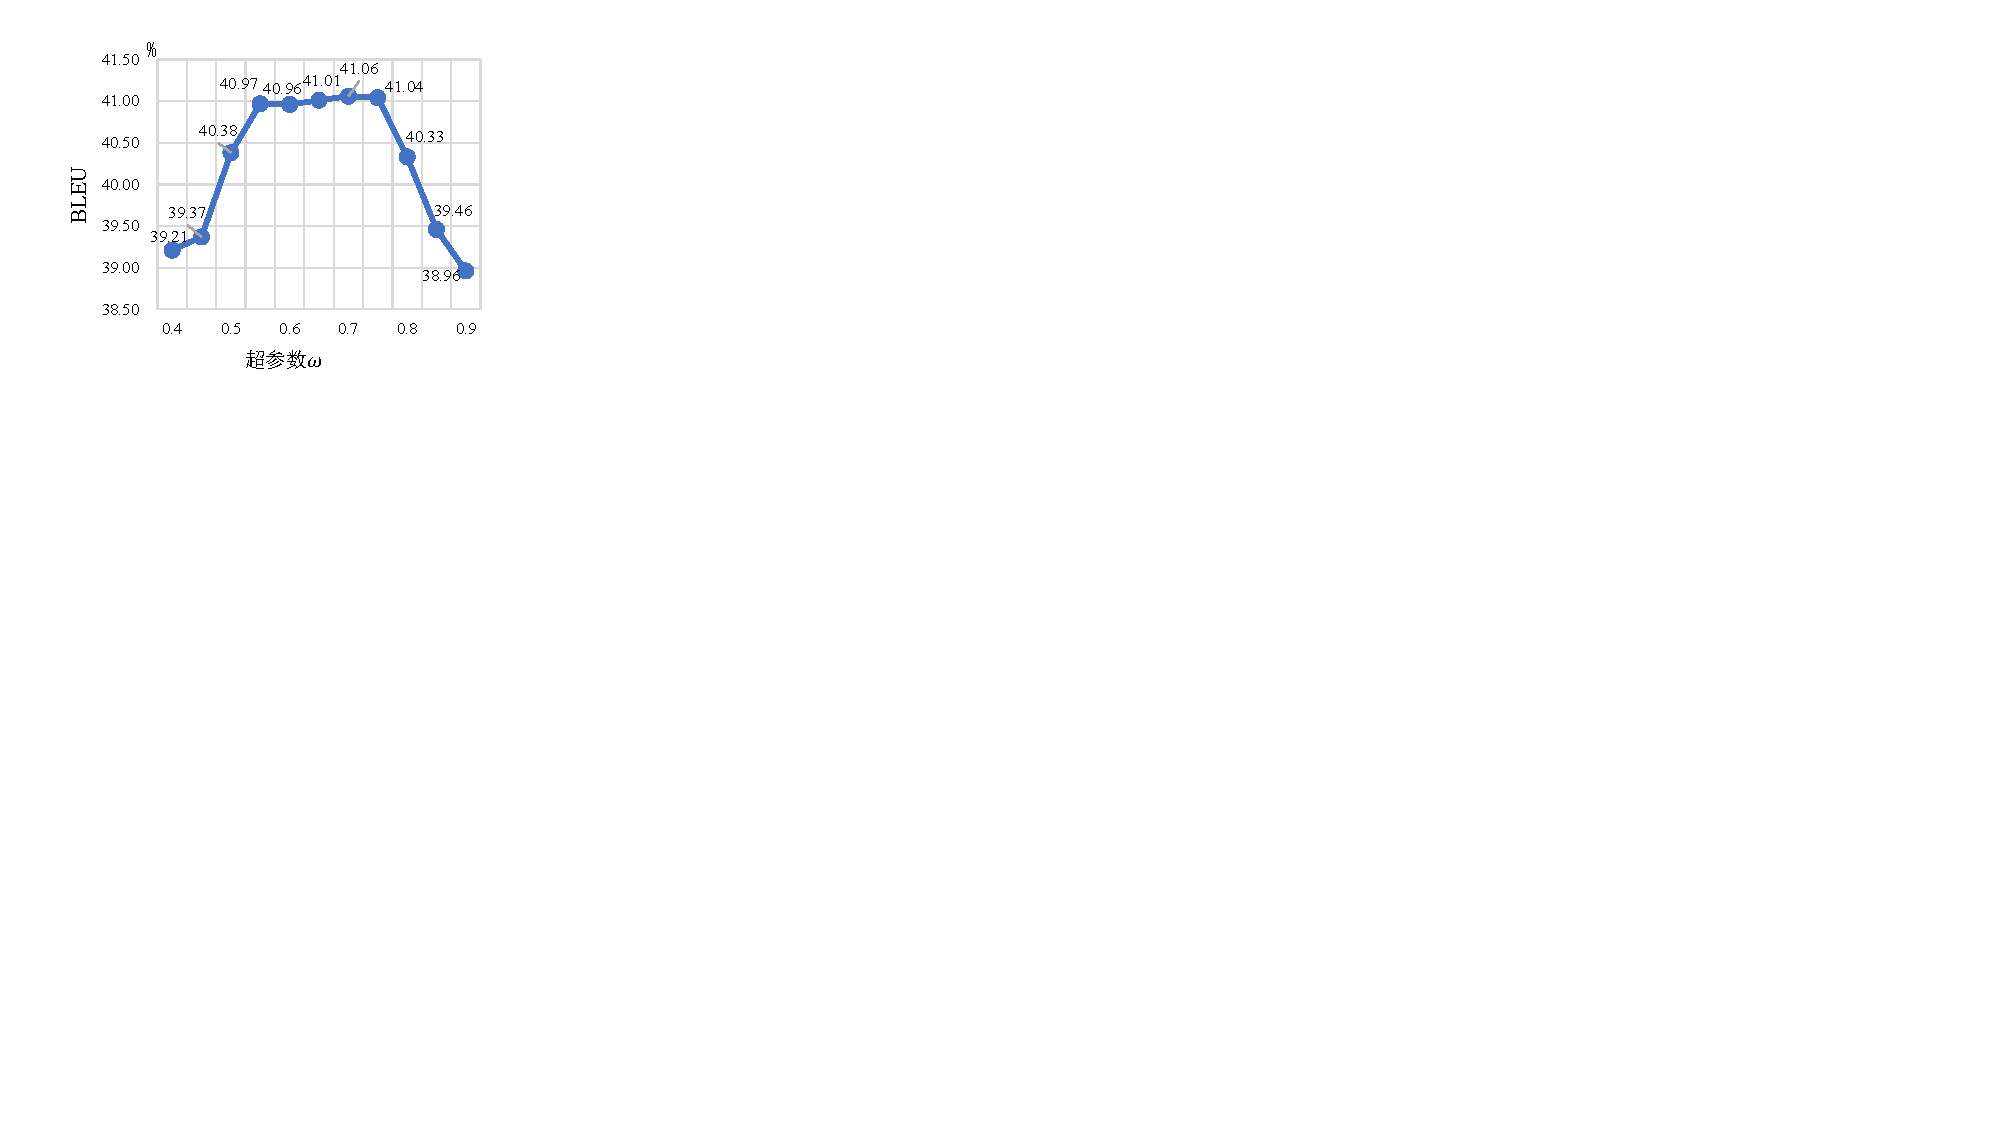
\includegraphics[scale=1.2]{Img/fig_4_searchw.pdf}
%    \bicaption{超参数$\omega$对CER-NMT翻译准确率的影响}{Effect of hyperparameter $\omega$ on translation accuracy of CER-NMT}
%    \label{fig:4_searchw}
%\end{figure}


\begin{figure}[!htbp]
    \centering
    \begin{subfigure}[b]{0.5\textwidth}
      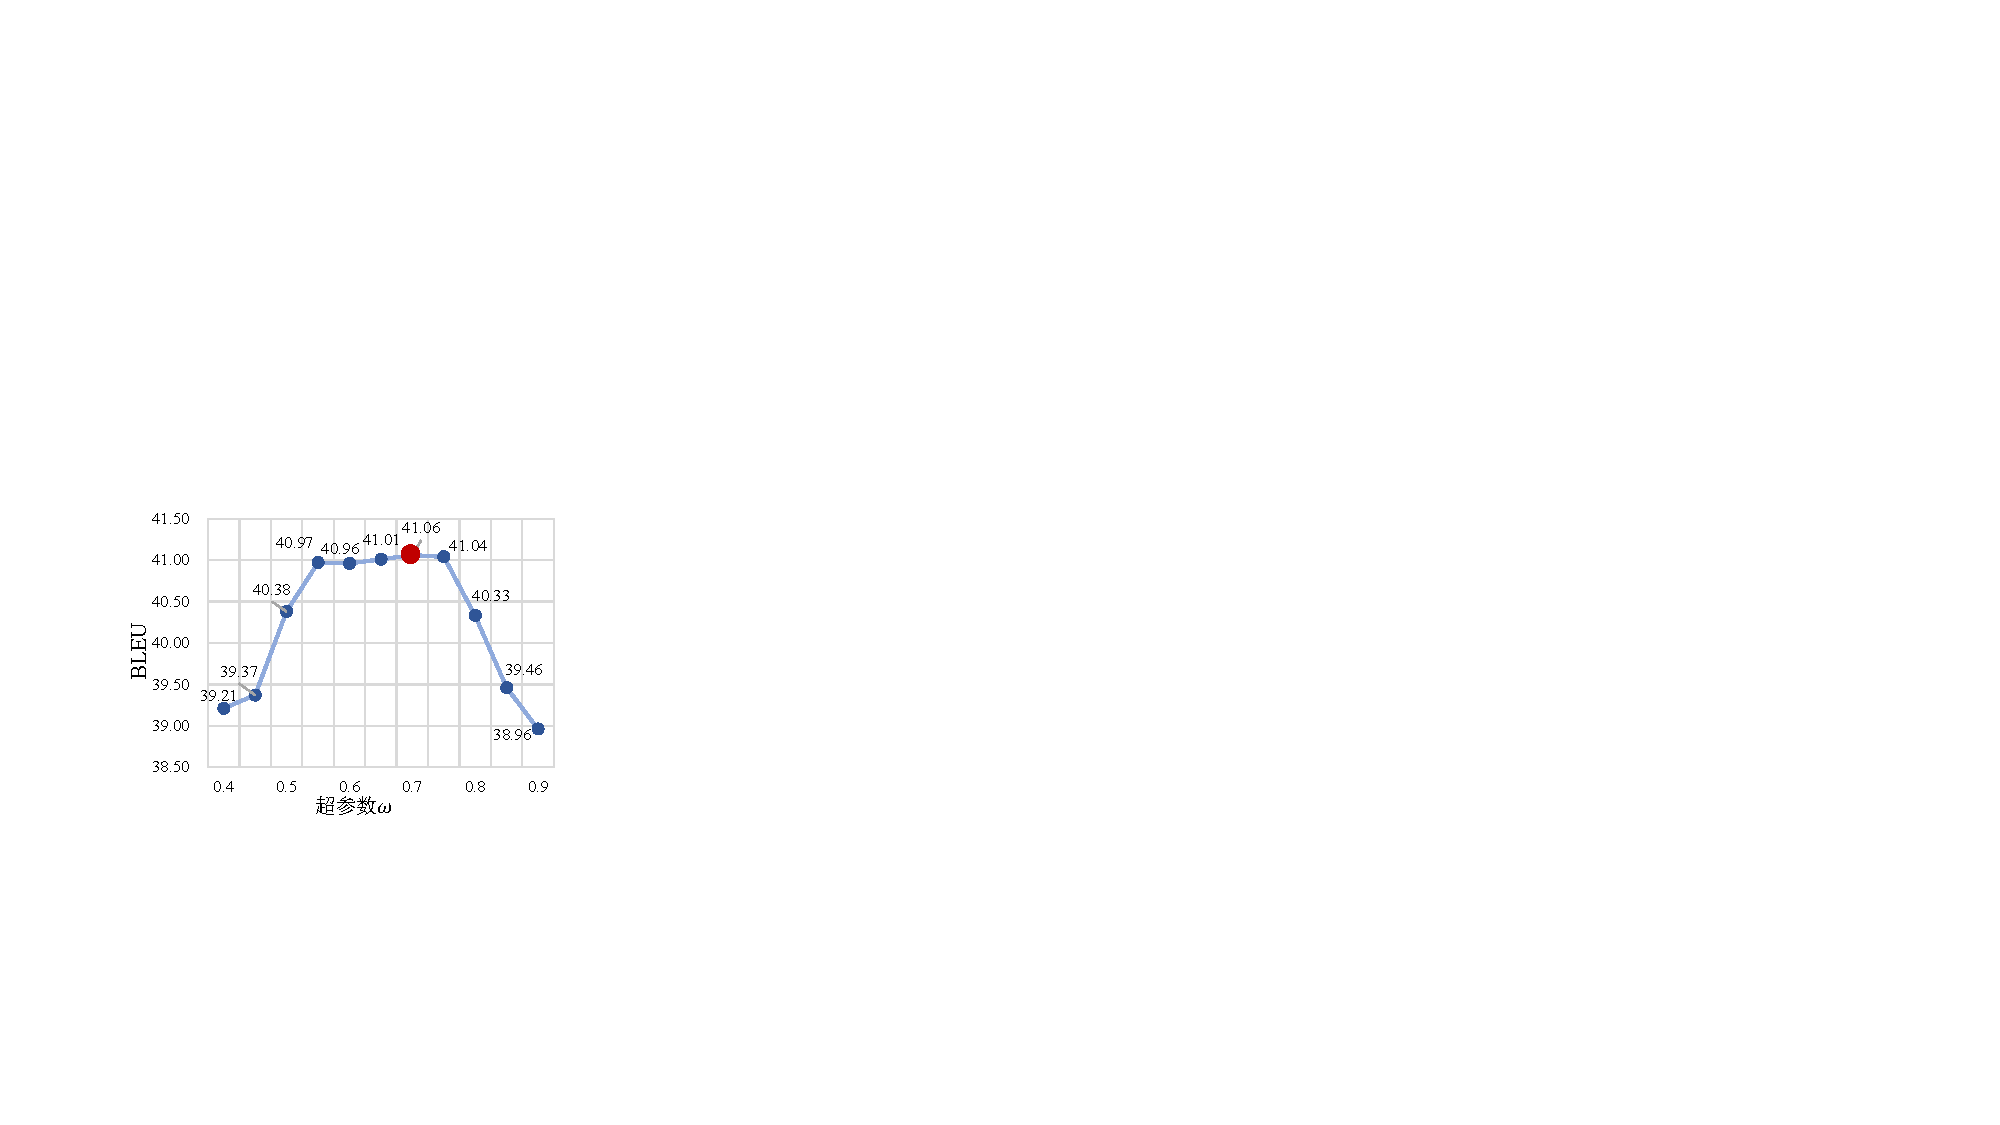
\includegraphics[width=\textwidth]{Img/fig_4_searchw_ende.pdf}
      \caption{英德翻译}
      \label{fig:4_searchw_ende}
    \end{subfigure}%
    ~% add desired spacing
    \begin{subfigure}[b]{0.5\textwidth}
      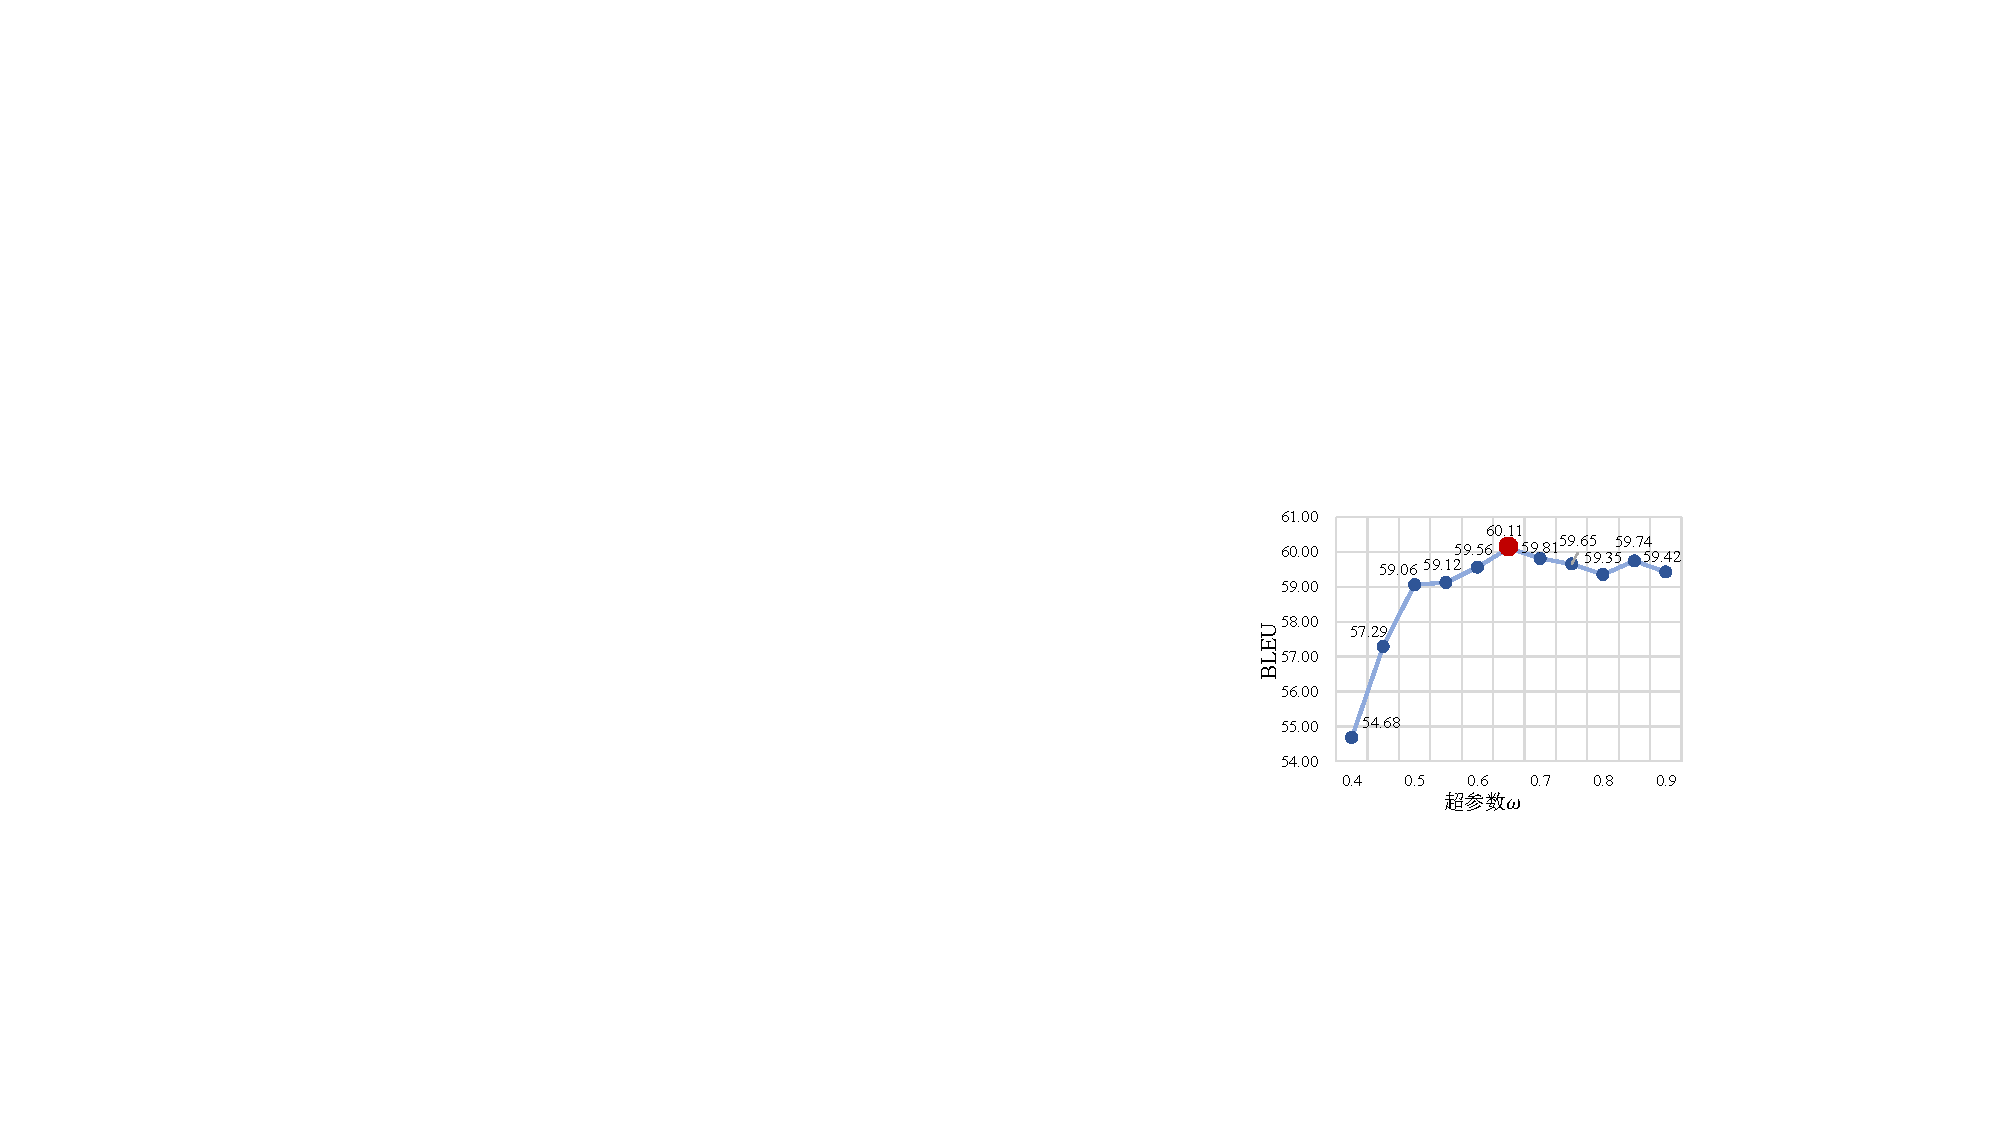
\includegraphics[width=\textwidth]{Img/fig_4_searchw_enfr.pdf}
      \caption{英法翻译}
      \label{fig:4_searchw_enfr}
    \end{subfigure}
    \\% line break
    \begin{subfigure}[b]{0.5\textwidth}
      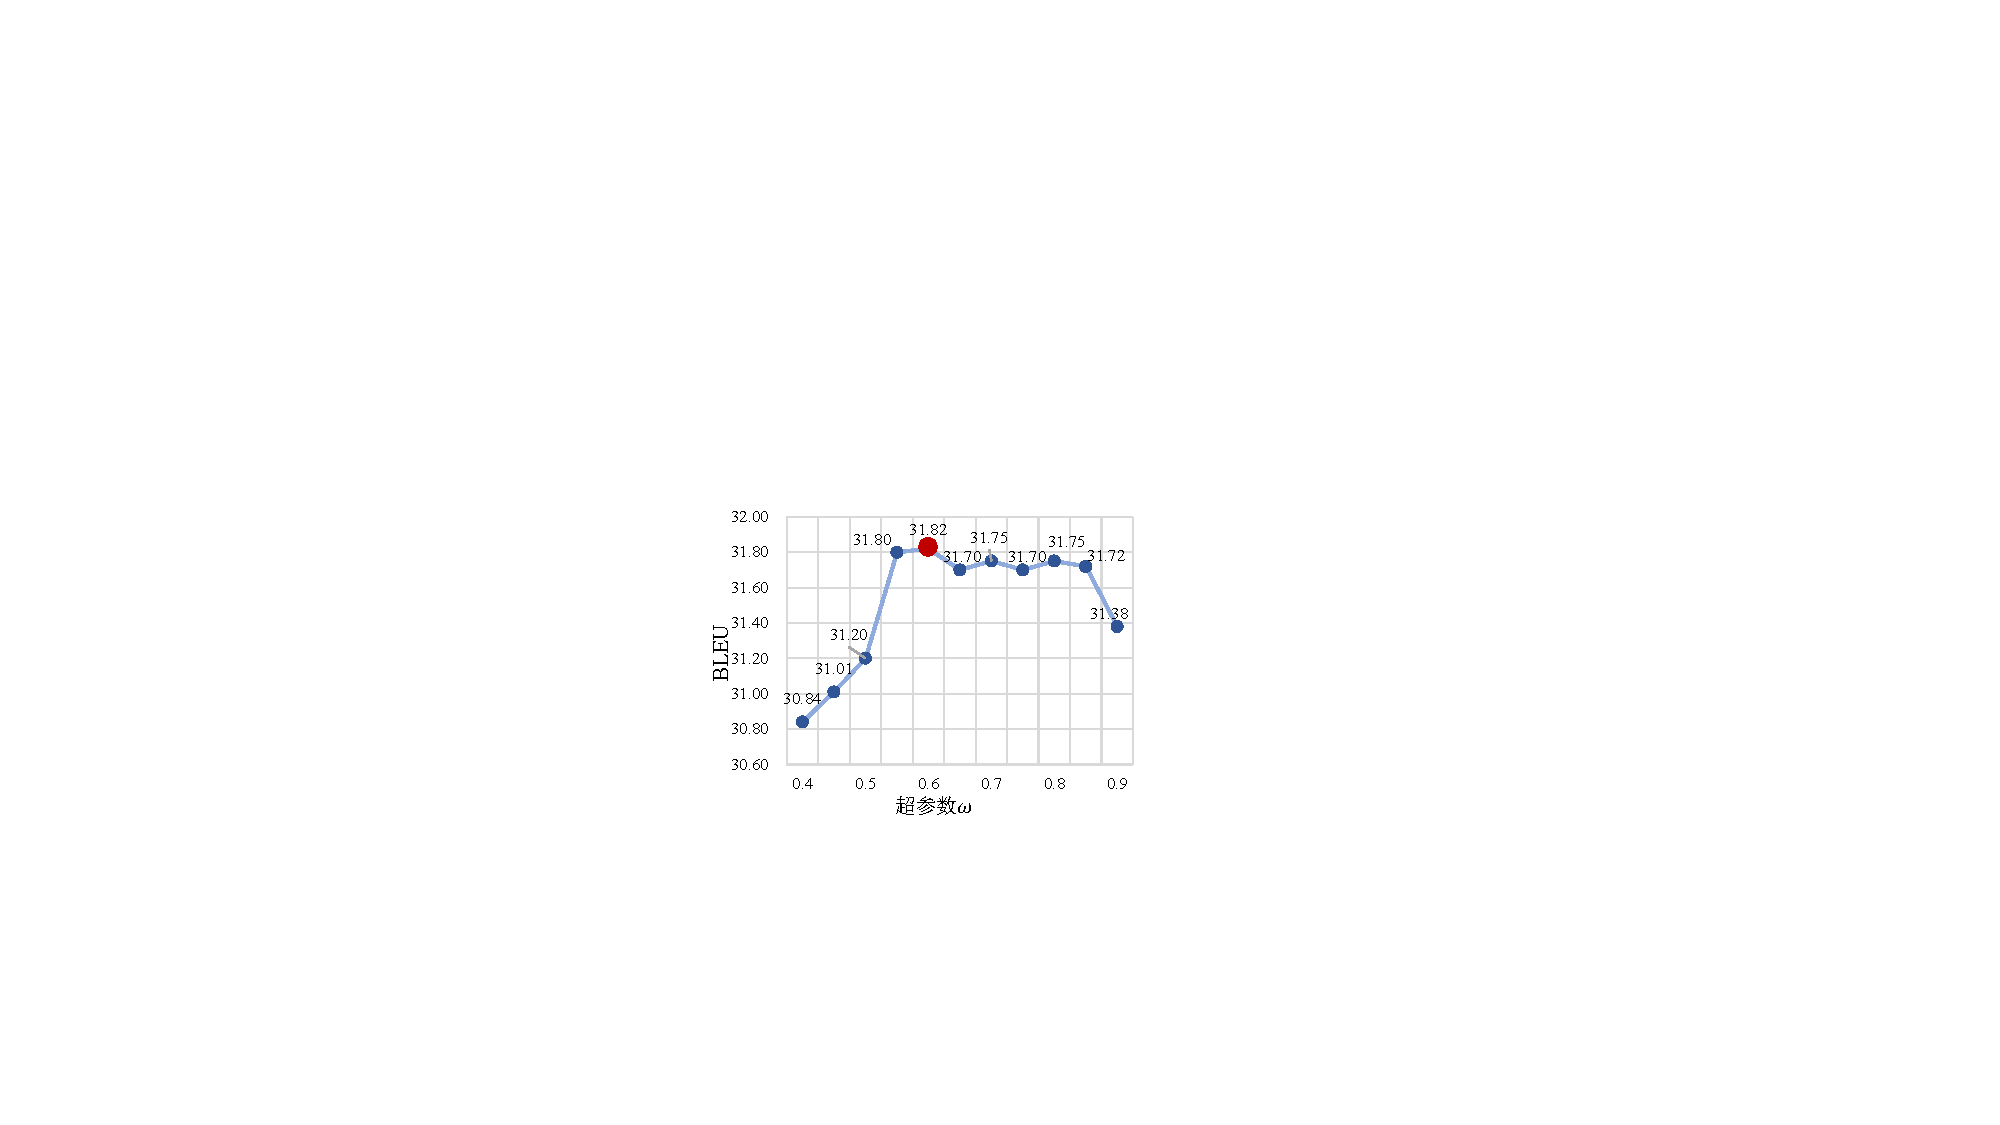
\includegraphics[width=\textwidth]{Img/fig_4_searchw_encs.pdf}
      \caption{英捷翻译}
      \label{fig:4_searchw_encs}
    \end{subfigure}%
    \bicaption{超参数$\omega$对CER-NMT翻译准确率的影响}{Effect of hyperparameter $\omega$ on translation accuracy of CER-NMT}
    \label{fig:4_searchw}
\end{figure}
如图\ref{fig:4_searchw}所示实验结果,横轴代表$\omega$从0.4以0.05为间隔增加至0.9,纵轴为CER-NMT模型在英德、英法和英捷三个翻译任务的验证集上的BLEU值。当$\omega=1.0$时,代表翻译任务的训练比例为$100\%$,此时是纯文本神经机器翻译。当$\omega=0.0$时,代表仅训练CER不做翻译。该图反映出,当$\omega \in [0.55,0.8]$时,模型普遍具有较好的BLEU值结果。超过这个范围时,CER-NMT的BLEU值将逐渐接近纯文本翻译模型。低于这个范围时,CER-NMT的翻译准确率发生了骤减。我们还测试了当$\omega=0.3$时的情况,此时英德翻译的BLEU值以骤减到9.86,英法骤减到8.62,英捷翻译骤减到3.94。以上实验结果说明在一个合适的范围内,CER方法能够帮助翻译模型提升翻译准确率。而这个范围应当使模型的训练过程主要以翻译任务为主以CER为辅。因此,本章选择$\omega=0.7$作为英德翻译模型的超参数,$\omega=0.65$作为英法翻译模型的超参数,$\omega=0.6$作为英捷翻译模型的超参数,即CER-NMT在验证集上达到最高的BLEU值时,作为后续试验中对超参数$\omega$的设置。


\subsection{翻译结果}
\label{sec:4_translation_results}


\begin{table}[!htbp]
    \bicaption{在Multi30K英德翻译、英法翻译和英捷翻译上的结果。}{Translation results on Multi30K EN-DE, EN-FR, EN-CS.}
    \label{tab:4_ende_enfr_encs}
    \centering
    \footnotesize% fontsize
    \setlength{\tabcolsep}{4pt}% column separation
    \renewcommand{\arraystretch}{1.2}%row space 
\begin{tabular}{ccccccccccc}
\hline
 \multirow{3}{*}{模型} & \multicolumn{6}{c}{英德翻译} & \multicolumn{2}{c}{英法翻译} & \multicolumn{2}{c}{英捷翻译} \\
\cmidrule(r){2-7} \cmidrule(r){8-9} \cmidrule(r){10-11}%\hline
       & \multicolumn{2}{c}{Test2016} & \multicolumn{2}{c}{Test2017} & \multicolumn{2}{c}{MSCOCO} & \multicolumn{2}{c}{Test2016} & \multicolumn{2}{c}{Test2016} \\
\cline{2-11}%\cmidrule(r){2-7} \cmidrule(r){8-9} %\cline{2-9}
              &    BLEU & Meteor &     BLEU & Meteor &     BLEU & Meteor &     BLEU & Meteor  &   BLEU & Meteor \\
\hline
\multicolumn{11}{c}{图片信息辅助式方法} \\
\hline
SerialAtt\pcite{libovicky2018input}      & 38.7 & 57.2 & - & - & - & - & 60.8 & 75.1 & 31.0 & 29.9 \\
DelMMT\pcite{ive2019distilling}           & 38.0 & 55.6 & - & - & - & - & 59.8 & 74.4 & - & -\\
GAMMT\pcite{liu2021gumbel}      & 39.2 & {\textbf{57.8}} & 31.4 & 51.2 & 26.9 & 46.0 & - & - & - & -\\
GMMT\pcite{yin2020novel}             & 39.8 & 57.6 & 32.2 & 51.9 & 28.7 & {\textbf{47.6}} & 60.9 & 74.9 & - & -\\
\hline
\multicolumn{11}{c}{图片信息增强式方法} \\
\hline
Imagination\pcite{elliott2017imagination}      & 36.8 & 55.8 & - & - & - & - & - & - & - & -\\
ImagiT\pcite{long2021generative}   & 38.6 & 55.7 & 32.1 & {\textbf{52.4}} & - & - & 59.9 & 74.3 & - & -\\
CTR-NMT             & 39.7 & 57.5 & {\textbf{32.9}} & 51.7 & {\textbf{29.1}} & 47.5 & 61.1 & 75.8 & 32.7 & 30.7\\
\hline
\multicolumn{11}{c}{本章所提方法} \\
\hline
Transformer\pcite{vaswani2017attention}             & 38.5 & 57.5 & 31.0 & 51.9 & 27.5 & 47.4 & 60.5 & 75.6 & 30.8 & 29.8 \\
CER-NMT          & {\textbf{40.2}} & {\textbf{57.8}} & 32.5 & 52.0 & 28.3 & 47.1 & {\textbf{61.9}} & {\textbf{76.4}} & {\textbf{32.9}} & {\textbf{31.2}}\\
\bottomrule
\end{tabular}
\end{table}

表\ref{tab:4_ende_enfr_encs}显示了采用CER方法的神经机器翻译系统的翻译结果。其中$\omega$按照4.1节的结论,针对英德翻译、英法翻译和英捷翻译的取值分别为0.7、0.65和0.6。对于VER、TER和TNER三个子任务,$\alpha$、$\beta$和$\gamma$的值分别设置为0.4、0.4和0.2。


表\ref{tab:4_ende_enfr_encs}中加粗项表示整列中的最佳结果。根据以上英德翻译、英法翻译和英捷翻译的实验结果可以得到以下结论:

%\begin{itemize}
%\item
(1)本章所提方法在Multi30K Test2016测试集的英德翻译、英法翻译和英捷翻译三个翻译对上取得了BLEU和Meteor值的最佳结果,并且在英德翻译Test2017测试集上的结果超过了多数模型的结果,并与其它模型的最佳结果相比差距很小。这说明CER方法能够有效提升NMT模型的翻译质量。

%\item
(2)CER-NMT在歧义词较多的Ambiguous MSCOCO上的表现并不理想,落后于GMMT和上一章的CTR-NMT两个模型。这是因为CER方法主要帮助翻译模型在训练阶段融合视觉信息,在测试阶段因为不需要输入图像使得模型无法借助视觉信息解决歧义词的问题。同理可以看到,CTR-NMT在Meteor上的提升也仅有0.1。这说明图片信息增强式的方法虽然能够提升模型的翻译质量,但也同样具有一定的局限性。例如文本中常见的歧义词问题或语义不完整问题,是需要利用图片信息辅助翻译模型进行解决。

(3)%\item
GMMT、CTR-NMT和CER-NMT均是采用视觉目标作为视觉输入的方法,其结果均优于采用完整图片输入的方法。理想的情况下,完整的图片包含的视觉信息更完整,对翻译带来的好处会更多。但是目前实验结果说明,在神经机器翻译中融合图片信息是非常困难的,需要为NMT模型提供更细粒度的视觉信息才能降低跨模态信息融合的难度,从而使模型更多地利用图片中的视觉信息。
%\end{itemize}

综合以上的实验结果,本章所提的跨模态实体重构方法能有效地提升机器翻译的质量。同时也说明了虽然图片信息增强式的翻译方法难以解决歧义词及语义不完整等问题,但是方法的有效性也体现了图片信息具有补全语义以外的其它作用。

\subsection{消融实验}
\label{sec:4_ablation_study}
为了探究VER、TER和TNER三个子任务对CER$-$NMT模型的影响,本节设置了12组消融实验。该实验是在Multi30K英德翻译的Test2016测试集上进行的。其中序号0代表上一节中CER-NMT的结果。序号1$-$3组各去掉一个子任务,并保持剩余子任务的训练权重。序号4$-$5组各去掉一个子任务,保持NMT的权重。序号7$-$9组各保留一个子任务,保持子任务的权重。序号10$-$12组保留一个子任务,保持NMT的权重。

\begin{table}[!htbp]
    \bicaption{在Multi30K Test2016英德翻译上消融实验结果}{Ablation study results on the EN-DE of Multi30K Test2016}
    \label{tab:4_ablation_study}
    \centering
    \footnotesize% fontsize
    \setlength{\tabcolsep}{4pt}% column separation
    \renewcommand{\arraystretch}{1.2}%row space 
\begin{tabular}{cccccc}
\hline
\multirow{2}{*}{序号} & NMT & VER & TER & TNER & \multirow{2}{*}{BLEU} \\
\cline{2-5}
   & $\omega$ & $(1-\omega) \times \alpha$ & $(1-\omega) \times \beta$ & $(1-\omega) \times \gamma$ & \\
\hline
0  & 0.70 & 0.12 & 0.12 & 0.06 & 40.2 \\
\hline
1  & 0.76 & 0.12 & 0.12 &  -   & 40.0 \\
2  & 0.82 & 0.12 & -    & 0.06 & 39.5 \\
3  & 0.82 & -    & 0.12 & 0.06 & 39.6 \\
\hline
4  & 0.70 & 0.15 & 0.15 & -    & 39.9 \\
5  & 0.70 & 0.20 & -    & 0.10 & 39.2 \\
6  & 0.70 & -    & 0.20 & 0.10 & 39.3 \\
\hline
7  & 0.88 & 0.12 & -    & -    & 38.8 \\
8  & 0.88 & -    & 0.12 & -    & 38.8 \\
9  & 0.94 & -    & -    & 0.06 & 39.0 \\
\hline
10 & 0.70 & 0.30 & -    & -    & 39.2 \\
11 & 0.70 & -    & 0.30 & -    & 39.4 \\
12 & 0.70 & -    & -    & 0.30 & 39.0 \\
\hline
\end{tabular}
\end{table}

实验结果如表\ref{tab:4_ablation_study}所示,其中“-”代表所对应的子任务被去掉,可以获得如下信息:

%\begin{itemize}
%\item
(1)序号1$-$6组各去掉了一个子任务,序号7$-$12组各仅保留一个子任务。从两组之间的对比可以看出,1$-$3的结果整体优于7$-$8,4$-$6的结果整体优于10$-$12,说明无论是保持子任务的训练比重不变还是保持翻译任务的训练比重不变,两个子任务组合的方式总是优于仅使用单一的子任务。其中,VER和TER的在序号1和4中的组合已经可以使翻译模型得到很好的结果。TNER对NMT的影响最小,但是依旧可以为NMT模型带来小幅度的提升。

%\item
(2)$\omega>0.8$的实验组2,3,7,8,9的结果与\ref{sec:4_omega}小节中的实验结果均说明减少跨模态任务至一定比重后,模型结果的BLEU值将逐渐趋近于纯文本翻译模型。因此在多任务训练阶段,不能因为翻译是主任务就将CER的比例调节的过低,保持两者的平衡更重要。

%\item
(3)与序号0中CER-NMT的实验结果相比可以说明,针对实体重构的VER和TER任务对翻译模型的性能影响最大,且这两个任务组合情况下的结果要优于单独使用的情况。相比之下,TNER同样可以为翻译性能带来一定的提升,但效果不如实体重构明显。综合以上,TER、VER和TNER三个子任务共同配合可以使翻译模型的性能达到最佳。
%\end{itemize}

消融实验的结果说明了本章所提的双向实体重构方法是有效的,视觉实体重构能够帮助文本实体重构进一步提升模型的翻译质量。文本非实体重构虽然为模型的性能提升带来的效果相对较小,但是将其与双向实体重构组合到一起可以得到CER方法的最佳效果。

\subsection{文本实体忠实度}
\label{sec:4_fidelity}
本章所提方法针对视觉实体与文本实体互相结合跨模态信息,再将视觉实体与文本上下文相融合。而这一过程中是以实体间的信息融合为主导的,在本章的消融实验中也证实了这一点。这使得视觉信息具有明确的作用方向。因此检验视觉信息是否对文本实体的翻译产生了影响成为了一个必要的环节。本节我们将尝试测量模型在解码生成目标单词时对源语言文本实体的忠实度,用于反映模型的行为变化。


Transformer的解码器采用的是交叉注意力机制,与一般的注意力机制类似的是,在解码过程中通过给源端的词不同的“权重”达到“关注”或“忽视”的作用。该“权重”体现了当前要解码的目标端单词对源端单词所提供信息的需求程度。因此,我们选择Transformer解码器最后一层交叉注意力权重的多头平均值,作为生成目标端词时对源端词的注意力“权重”,并定义该“权重”为忠实度(fidelity),用于量化生成目标端文本实体时对源端文本实体的忠实程度。\ref{sec:4_dataset}小节中提到,源端的文本实体是通过文本分析工具提取得到。本节中所要确定的目标端文本实体是通过fast-align\pcite{dyer2013simple}对齐工具对齐源端与目标端单词得到的。为了得到一个较好的对齐结果,我们将测试集与训练集拼接后训练对齐模型。


\begin{figure}[!htbp]
    \centering
    \begin{subfigure}[b]{0.5\textwidth}
      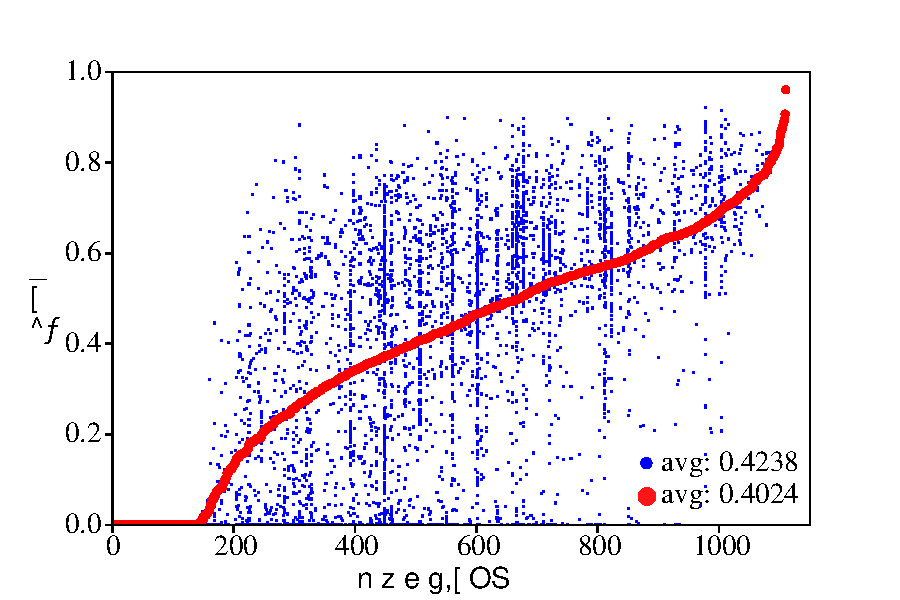
\includegraphics[width=\textwidth]{Img/fig_4_fidelity_base.pdf}
      \caption{Transformer}
      \label{fig:4_fidelity_base}
    \end{subfigure}%
    ~% add desired spacing
    \begin{subfigure}[b]{0.5\textwidth}
      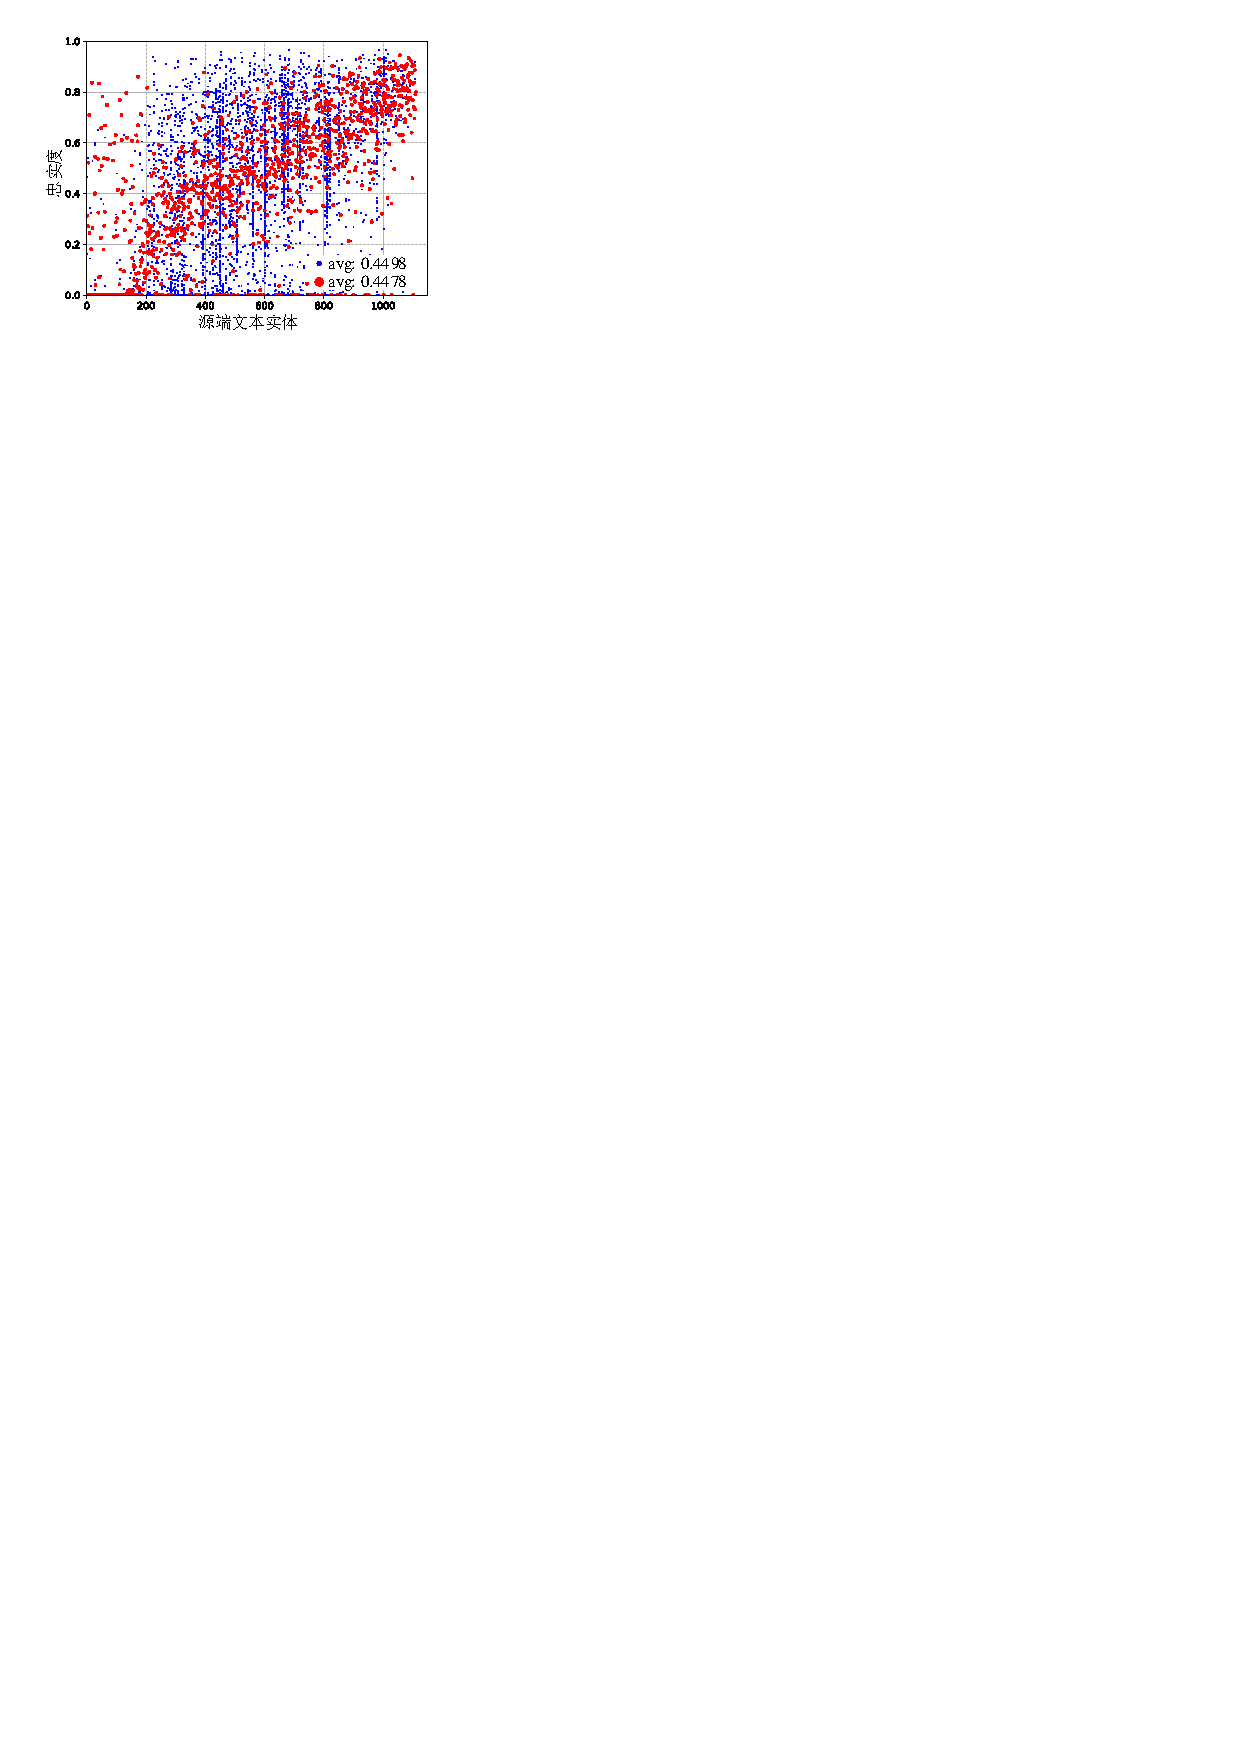
\includegraphics[width=\textwidth]{Img/fig_4_fidelity_cer_baseorder.pdf}
      \caption{CER-NMT}
      \label{fig:4_fidelity_cer_baseorder}
    \end{subfigure}
    \\% line break
    \begin{subfigure}[b]{0.5\textwidth}
      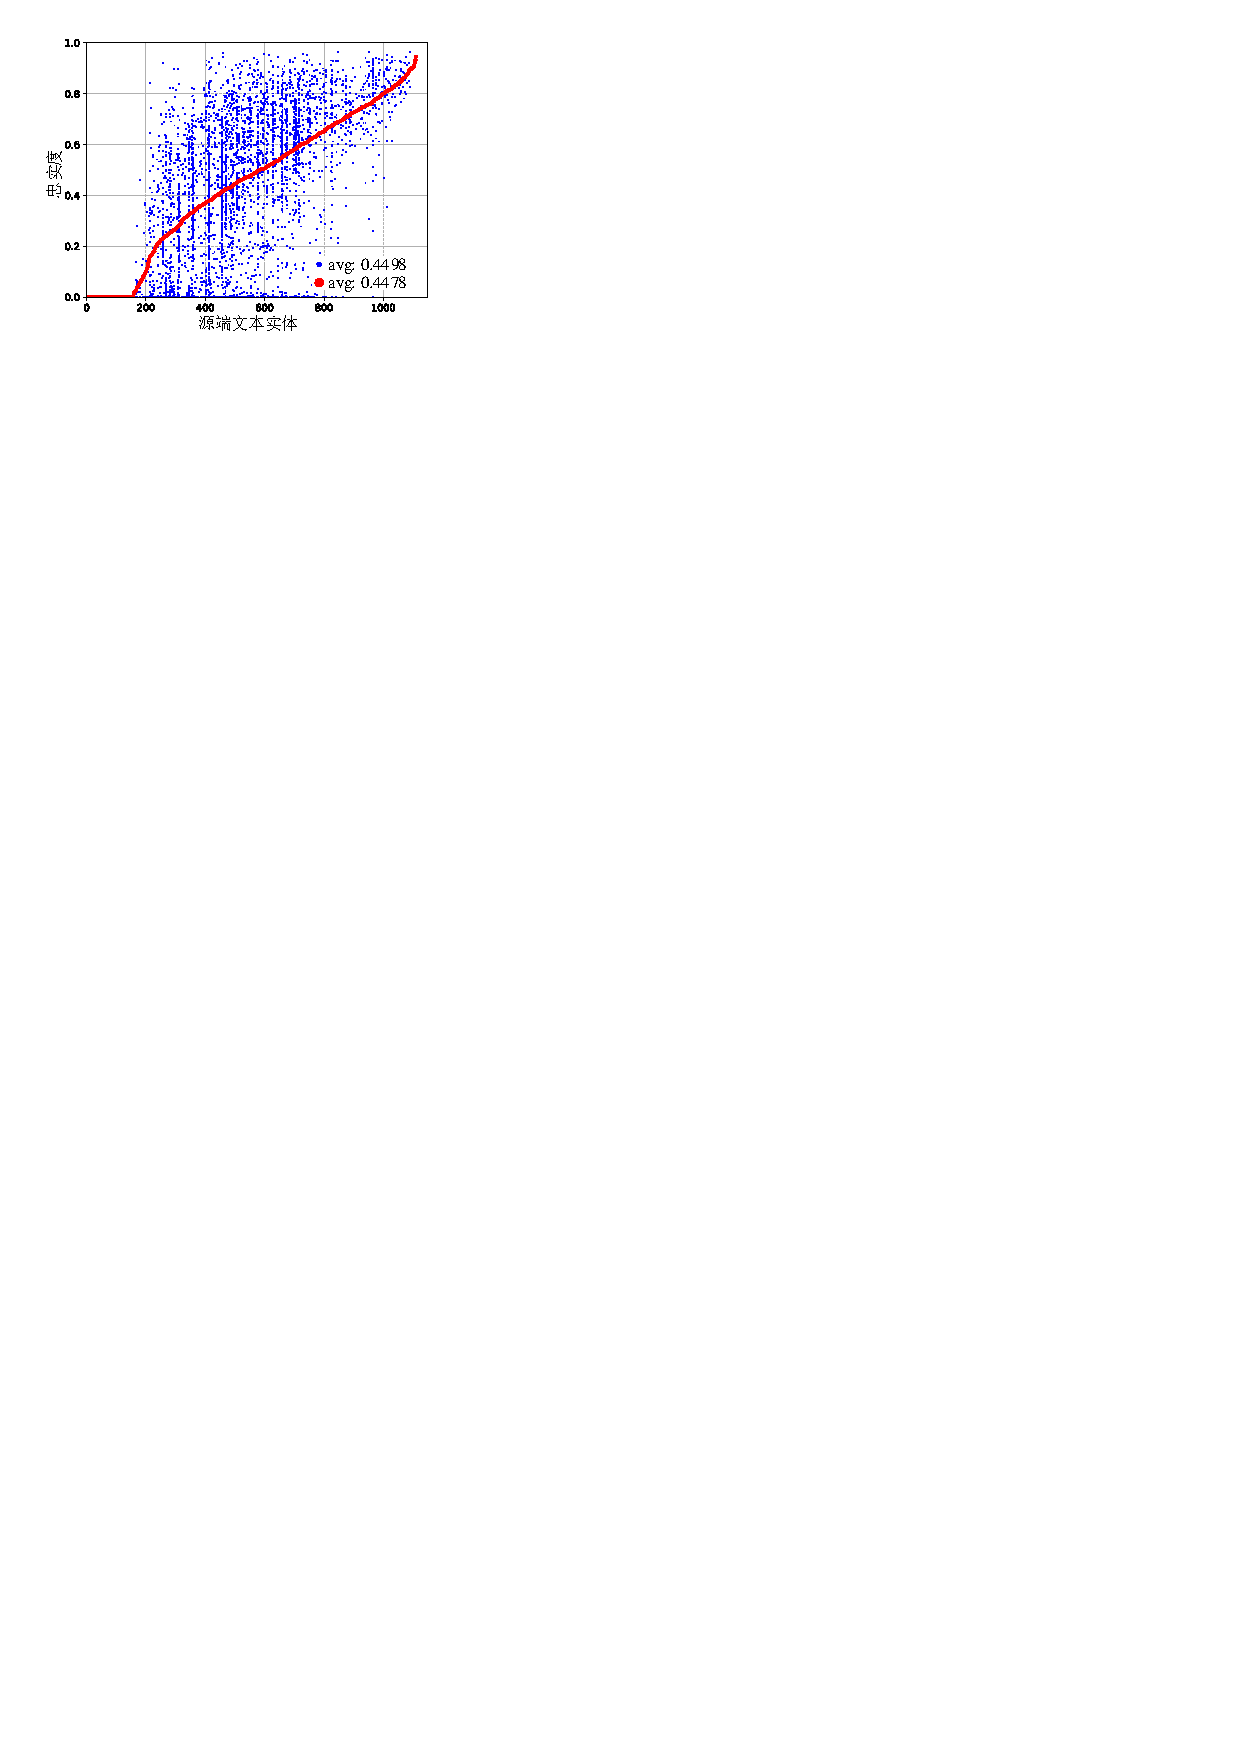
\includegraphics[width=\textwidth]{Img/fig_4_fidelity_cer_selforder.pdf}
      \caption{实体重排序的CER-NMT}
      \label{fig:4_fidelity_cer_selforder}
    \end{subfigure}%
    ~% add desired spacing
    \begin{subfigure}[b]{0.5\textwidth}
      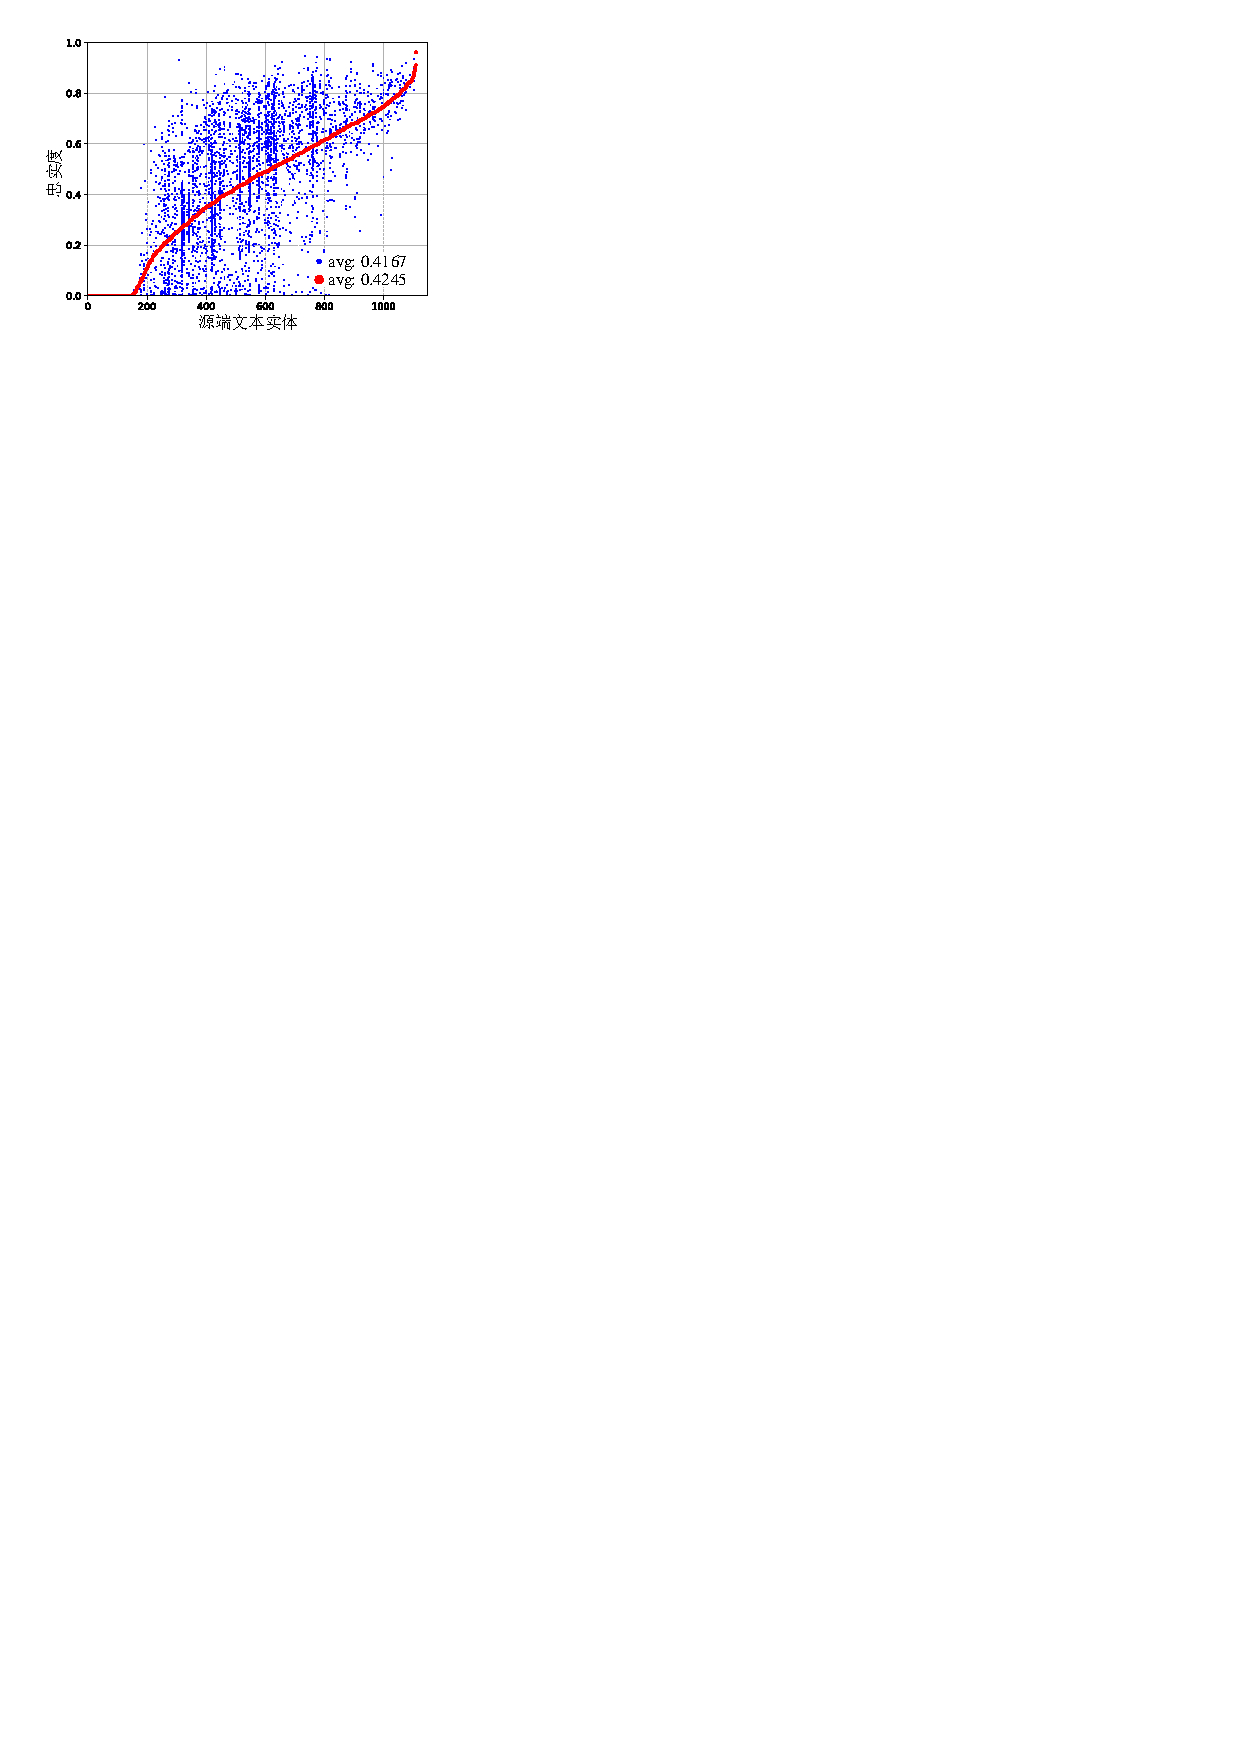
\includegraphics[width=\textwidth]{Img/fig_4_fidelity_tner.pdf}
      \caption{TNER-NMT}
      \label{fig:4_fidelity_tner}
    \end{subfigure}
    \bicaption{文本实体在不同模型下的忠实度}{The fidelity of textual entities on different models}
    \label{fig:4_fidelity}
\end{figure}
实验结果如图\ref{fig:4_fidelity}所示,图中横轴代表测试集中源语言文本实体以某种方式的排序,纵轴为范围从0到1的忠实度。每个小像素点代表一个源端文本实体在一个翻译句子样本中对应目标端文本实体的注意力权重值,即实体词忠实度。大圆点代表每个实体词的平均忠实度。图\ref{fig:4_fidelity}(a)为纯文本Transformer的测试结果,横轴为测试集中的1110个源端文本实体,并按照平均忠实度由小到大排序。图\ref{fig:4_fidelity}(b)为CER-NMT与图\ref{fig:4_fidelity}(a)横轴词序保持一致的结果,图\ref{fig:4_fidelity}(c)为CER-NMT对实体词重排序后的结果。图\ref{fig:4_fidelity}(d)为\ref{sec:4_ablation_study}节序号12仅设置TNER,且保持翻译任务训练比例为70\%不变的模型。图中“avg”代表平均值。从4个图的对比中可以得到以下信息:

%\item
(1)图中忠实度为0的横线部分代表对齐模型无法在目标端句子中找到对应的实体词。因此这些词的忠实度为0。

%\item
(2)图\ref{fig:4_fidelity}(b)相比于图\ref{fig:4_fidelity}(a)存在更多靠近1.0的小像素点。从图\ref{fig:4_fidelity}(c)中的均值结果(avg)可以看到,小像素点的均值从0.4238提升至0.4498,大圆点的均值从0.4024提升至0.4478,均具有较明显的提升。该数值结果表明CER方法能够显著地提升模型在翻译过程中对源语言文本实体的忠实度。

%\item
(3)图\ref{fig:4_fidelity}(c)经过重排序实体的顺序后,可以更直观地从曲线的趋势看出采用CER方法所带来的忠实度的提升。

%\item
(4)TNER对文本上下文和视觉实体进行句子级的语义融合,可以观察到图\ref{fig:4_fidelity}(d)相对于图\ref{fig:4_fidelity}(a)有提升也有降低,这说明VER和TER才是帮助提升文本实体忠实度的主要因素,针对非实体的重构方法所带来的翻译性能提升无法没有显著地体现在实体忠实度的提升上。
%\end{itemize}

以上结果表明,CER方法通过融入视觉信息的方式,增加了翻译模型在翻译过程中对源语言文本实体的忠实度,从而使得翻译结果得到了进一步的提升。该实验同样表明本章的双向跨模态实体重构方法是有效可行的,该显式跨模态信息融合方法使得模型更具备可解释性,视觉信息的作用方式更有迹可循。

\subsection{基于词频的翻译准确率统计}
\label{sec:4_freq_acc}


\begin{figure}[!htbp]
    \centering
    \begin{subfigure}[b]{0.5\textwidth}
      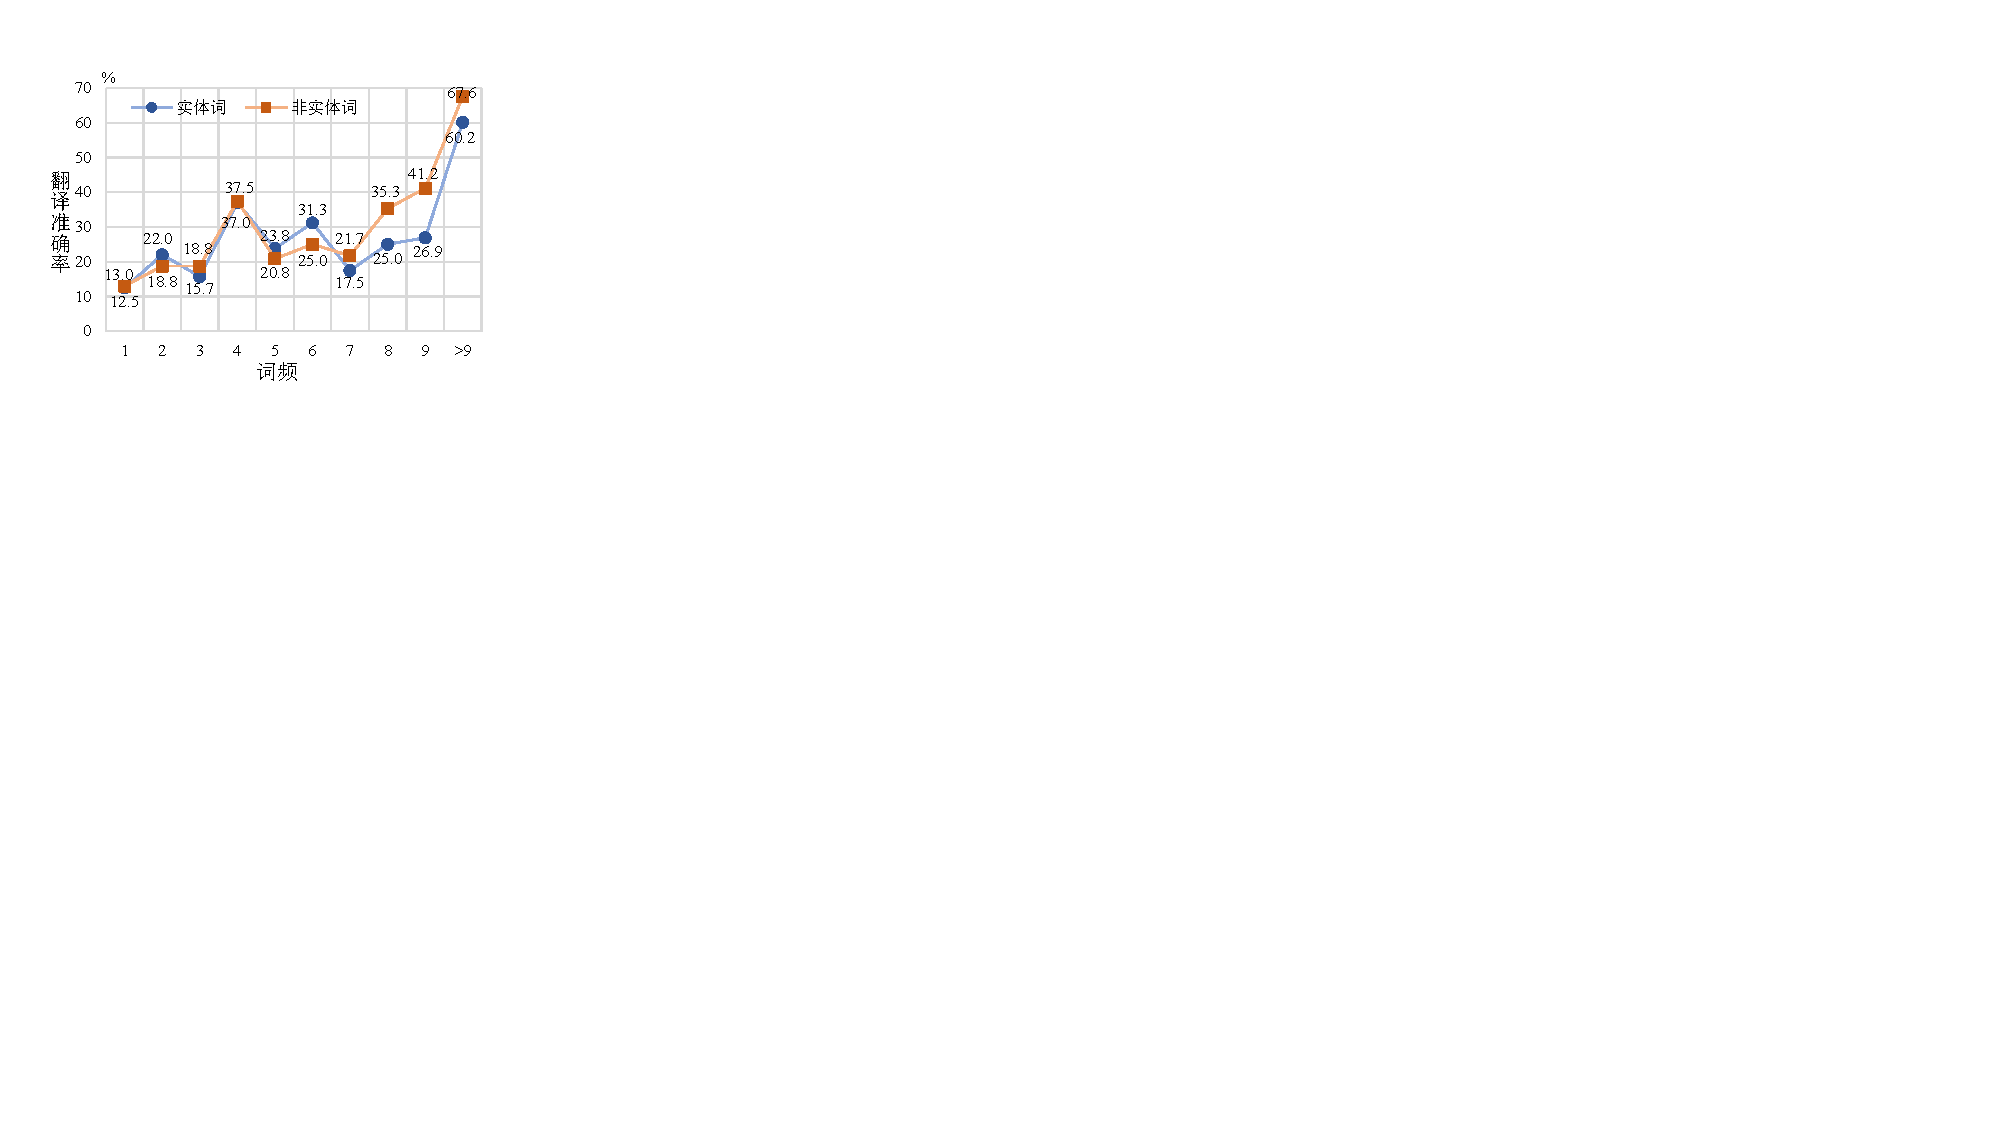
\includegraphics[width=\textwidth]{Img/fig_4_freq_acc_transformer.pdf}
      \caption{Transformer}
      \label{fig:4_freq_acc_transformer}
    \end{subfigure}%
    ~% add desired spacing
    \begin{subfigure}[b]{0.5\textwidth}
      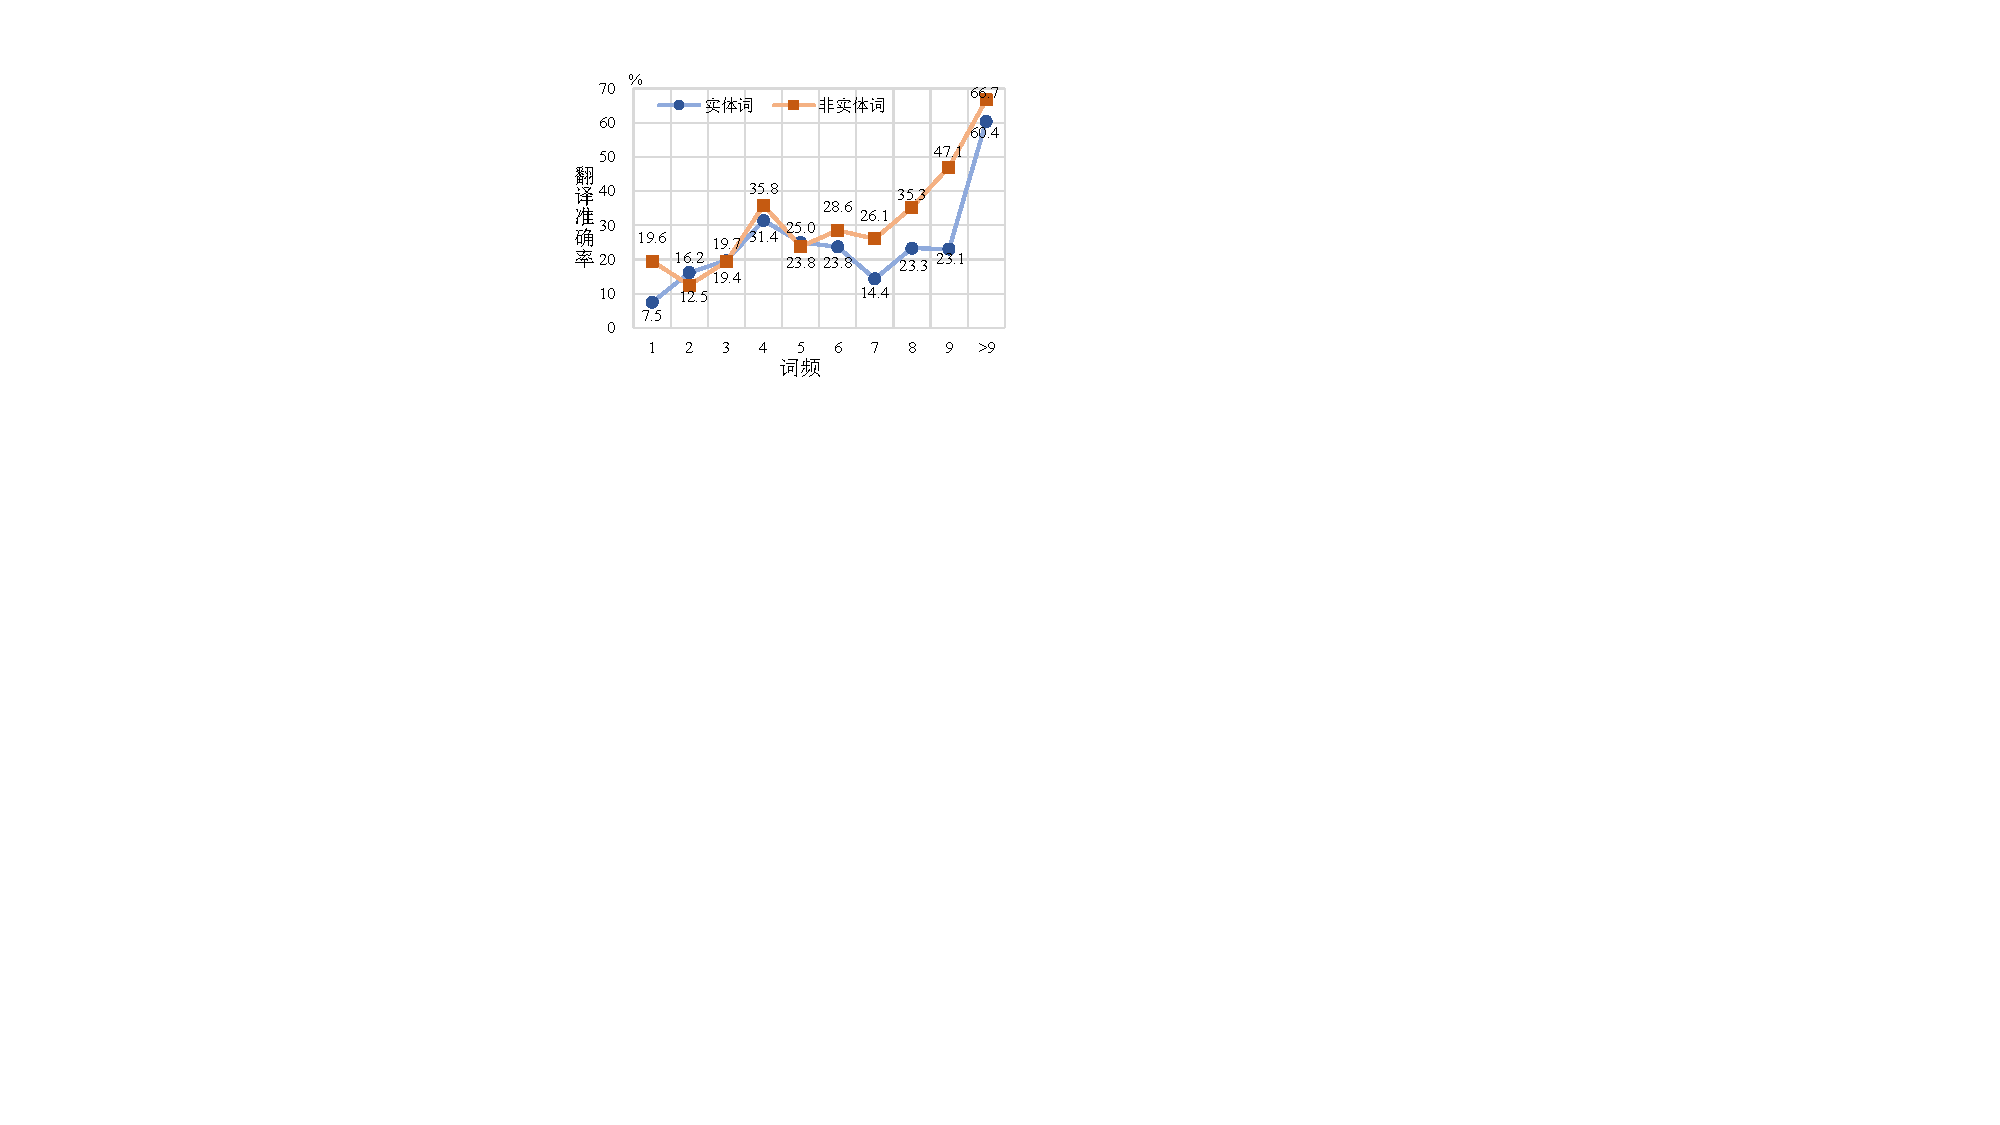
\includegraphics[width=\textwidth]{Img/fig_4_freq_acc_tner.pdf}
      \caption{TNER-NMT}
      \label{fig:4_freq_acc_tner}
    \end{subfigure}
    \\% line break
    \begin{subfigure}[b]{0.5\textwidth}
      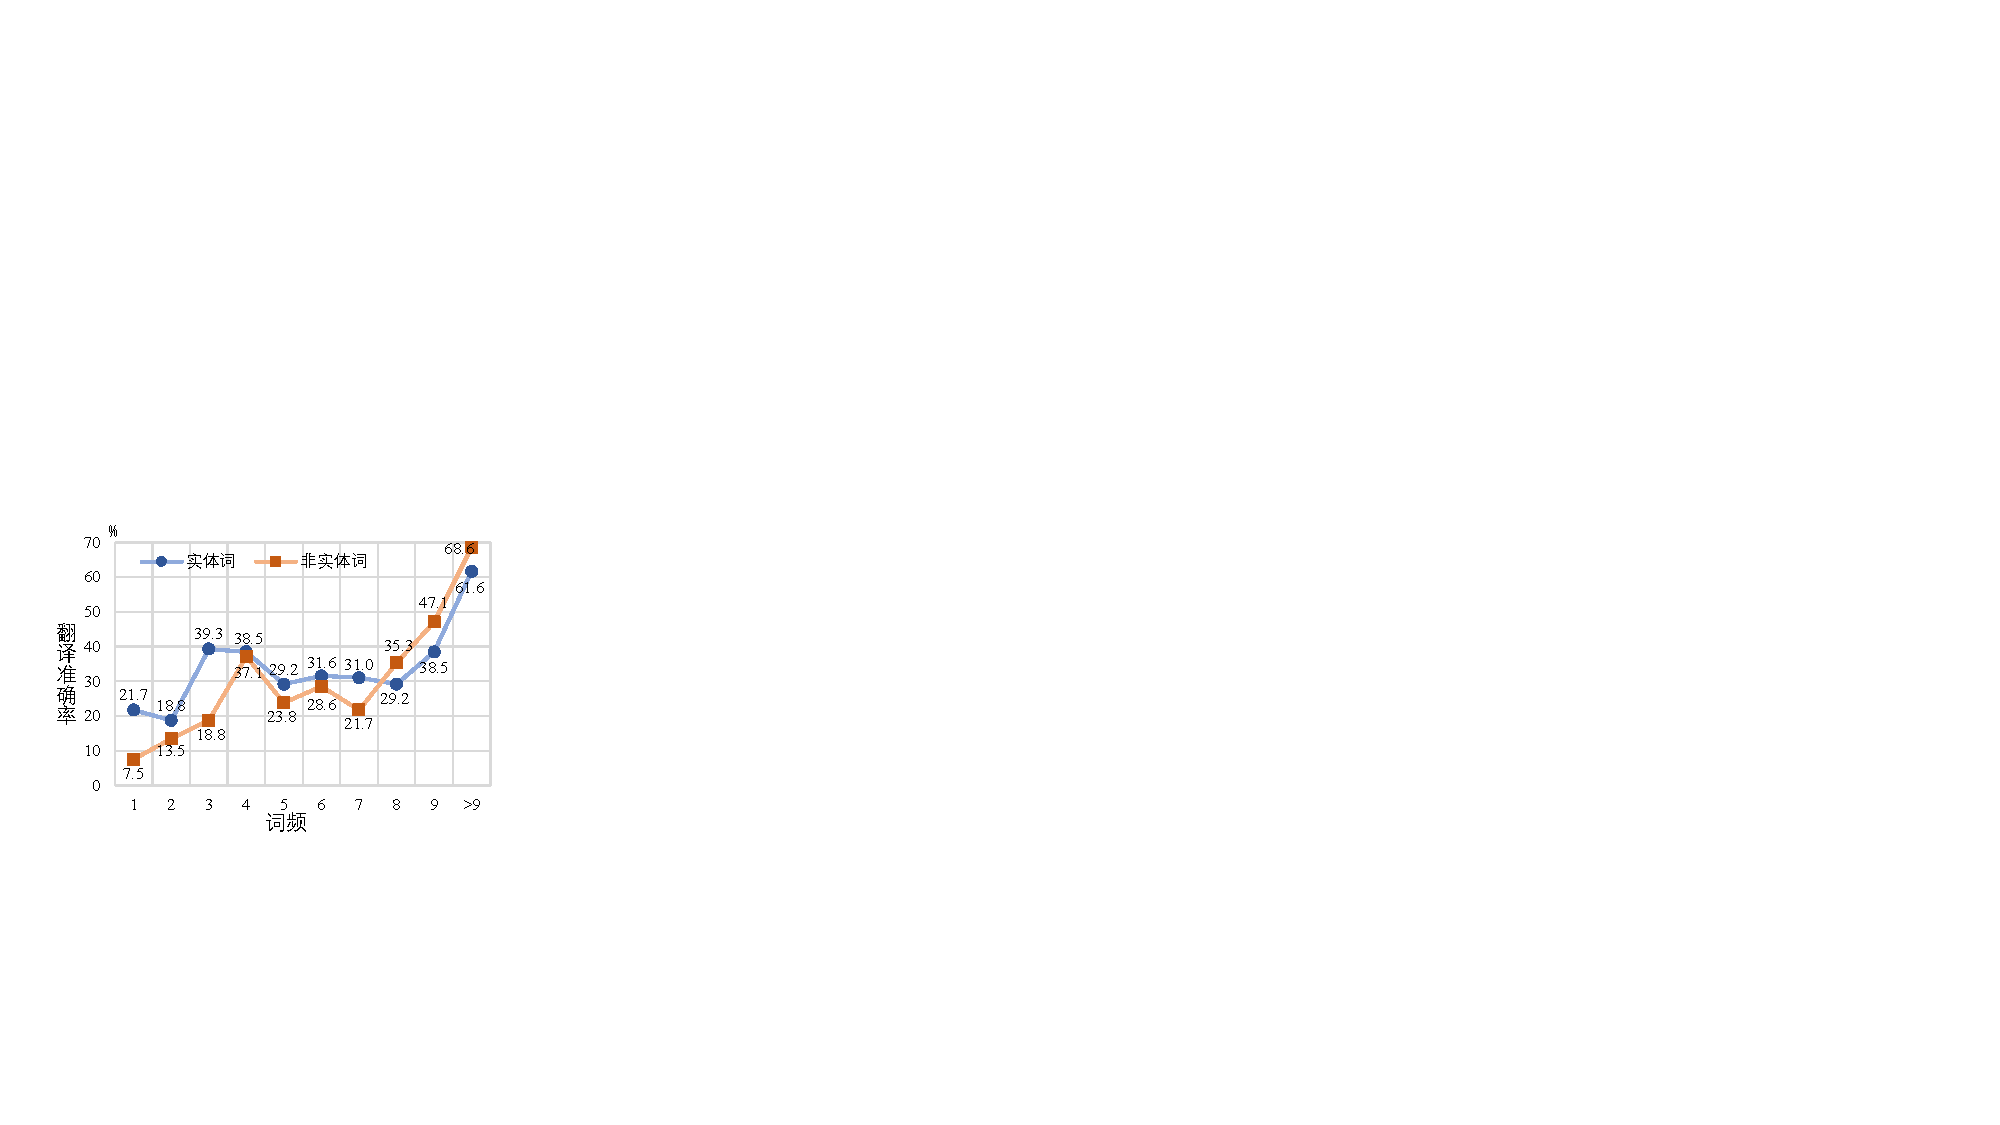
\includegraphics[width=\textwidth]{Img/fig_4_freq_acc_cer.pdf}
      \caption{CER-NMT}
      \label{fig:4_freq_acc_cer}
    \end{subfigure}%
    ~% add desired spacing
    \begin{subfigure}[b]{0.5\textwidth}
      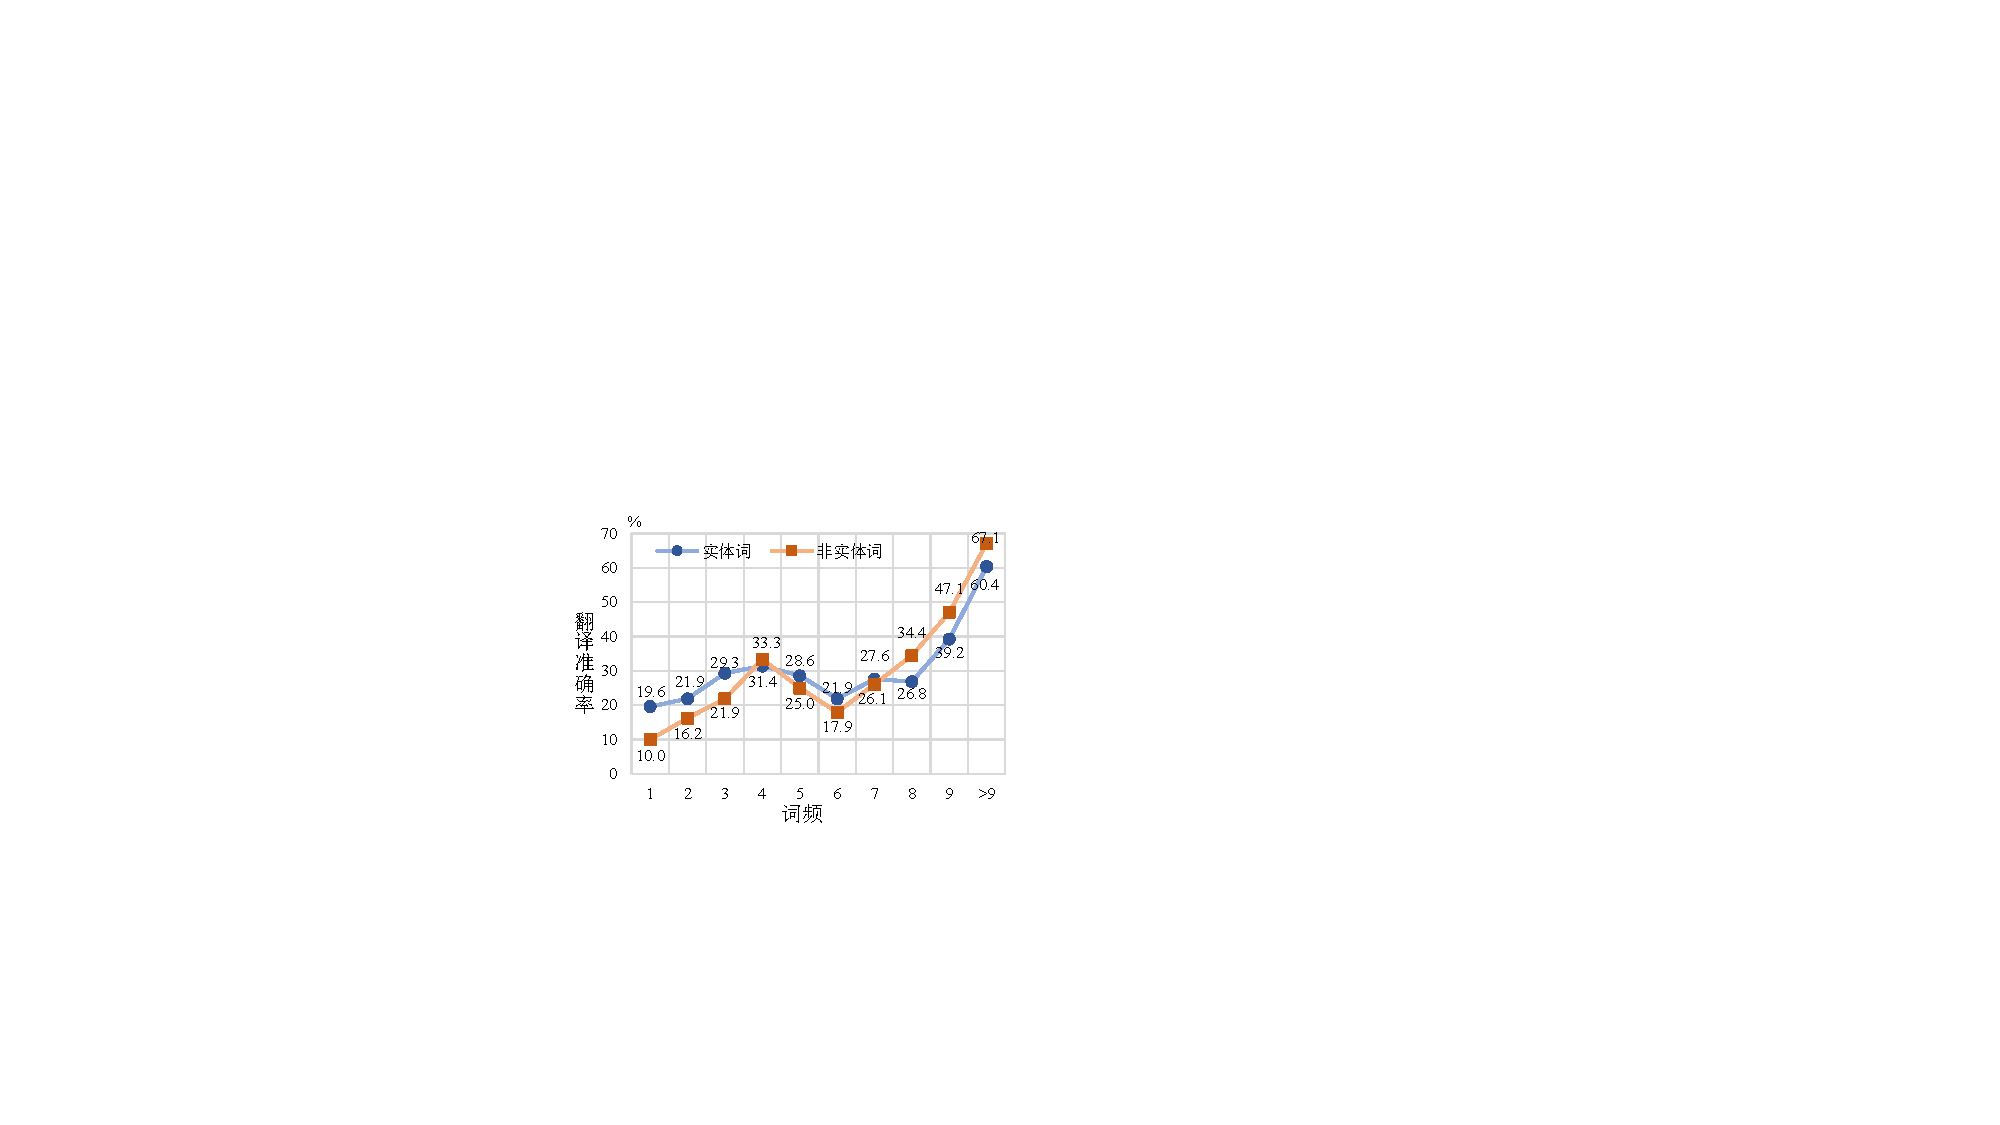
\includegraphics[width=\textwidth]{Img/fig_4_freq_acc_ctr.pdf}
      \caption{CTR-NMT}
      \label{fig:4_freq_acc_ctr}
    \end{subfigure}
    \bicaption{\centering{实体词和非实体词在不同词频下的翻译准确率}}{Translation accuracy of entity and none-entity words in different word frequencies}
    \label{fig:4_freq_acc}
\end{figure}
上一节通过统计翻译过程中目标语言的文本实体相对于源语言的文本实体的忠实度,反映实体重构方法对翻译过程带来的影响。并发现,文本实体在翻译过程中得到了更多的重视。
为了进一步反映重构方法对神经机器翻译带来的影响,我们首先统计了文本实体在所使用数据中的占比情况。统计发现,文本实体占训练集和测试集单词总数的32.6\%,文本实体在词表中的占比为59.9\%,文本实体平均词频为20.2,词频的中位数为2。根据该统计结果不难发现,大部分的实体词的词频小于等于2,反映出实体词主要分布于低频词中。这也说明了在神经机器翻译中,针对实体词的翻译更加困难。

为了探究本章的实体重构方法为文本实体的翻译带来的影响,本节统计了文本实体的翻译准确率随词频变化的统计结果。文本实体的翻译准确率的计算延续了上一节对齐原文与译文之间单词的方法。首先需要将原文与参考译文进行词对齐,从而得到在每个句子中,每个单词在翻译过程中需要对齐到目标语言句子中的哪个单词。然后将神经机器翻译系统的翻译结果同样对齐到原文,从而得到该翻译系统将源语言句子中的每个词对齐到了译文中的哪个单词。通过对比所对齐的单词是否相同的方式,来判断当前单词的翻译是否正确。

图\ref{fig:4_freq_acc}展示了针对纯文本Transformer、本章的TNER-NMT、本章的CER-NMT以及上一章的CTR-NMT四个神经机器翻译系统在不同词频下的文本实体和非文本实体的翻译准确率统计情况。该统计结果基本满足随着词频的升高翻译准确率也随着升高的规律。词频较低的情况下,单词的翻译准确率的波动很大,这能够反映出模型对出现次数较少的单词的翻译置信程度较低。值得注意的是,CER-NMT和CTR-NMT都采用了明确的视觉信息作用方法,将视觉目标信息作用到文本实体上。因此这两种方法都对文本实体的翻译有较强的提升作用,这在图\ref{fig:4_freq_acc}(c)和\ref{fig:4_freq_acc}(d)中反映在文本实体的翻译准确率在词频低于8时普遍高于文本非实体。当词频大于等于8时,虽然非实体的翻译准确率明显高于实体,但它们之间的差距明显小于Transformer和TNER-NMT的结果,而这一规律与上一章的\ref{sec:3_entity_analysis}的分析结果是一致的。这进一步说明了,虽然实体词在整体上的翻译准确率低于非实体词,但是在低频词部分,因实体重构带来的强化作用,使低频实体词的翻译准确率已经超过了低频非实体词。


\begin{table}[!htbp]
    \bicaption{\centering{低频词与高频词的翻译准确率统计情况}}{Statistics about the translation accuracy of low-frequency words and high-frequency words}
    \label{tab:4_freq_acc}
    \centering
    \footnotesize% fontsize
    \setlength{\tabcolsep}{4pt}% column separation
    \renewcommand{\arraystretch}{1.2}%row space 
    \begin{tabular}{c|cc|cc|cc|cc}
    \hline
    %& \multicolumn{4}{c}{文本实体} & \multicolumn{4}{c}{文本非实体} \\
    %& Transformer & TNER-NMT & CER-NMT & CTER-NMT & Transformer & TNER-NMT & CER-NMT & CTER-NMT \\
    & \multicolumn{2}{c}{Transformer} & \multicolumn{2}{c}{TNER-NMT} & \multicolumn{2}{c}{CER-NMT} & \multicolumn{2}{c}{CTR-NMT} \\\cline{2-9}
      & 实体 & 非实体 & 实体 & 非实体 & 实体 & 非实体 & 实体 & 非实体 \\\hline
    低频词(<8) & 22.8 & 22.2 & 19.7 & 23.7 & 30.0 & 21.6 & 25.7 & 21.5 \\
    高频词(>=8)& 37.4 & 48.0 & 35.6 & 49.7 & 43.1 & 50.3 & 42.2 & 49.5 \\
     \hline
    \end{tabular}%
\end{table}%

图\ref{fig:4_freq_acc}反映出词频为8时,词的翻译准确率出现了一个明显的分水岭。因此,我们将词频低于8的单词作为低频词,大于等于8的为高频词,得到表\ref{tab:4_freq_acc}关于低频词和高频词的翻译准确率统计结果。从该结果中可以看出,采用显式融合方式的CER-NMT和CTR-NMT的实体词翻译准确率在低频词和高频词上均有较明显的提升,非实体词的差距并不大。CER-NMT相比于上一章的CTR-NMT有小幅度的提升,说明增加了视觉实体重构的双向实体重构方案相比于单独使用文本重构能够为实体词的翻译带来更进一步的性能提升。TNER-NMT采用了30\%的文本非实体重构,这也反映在表\ref{tab:4_freq_acc}中其低频非实体词的翻译准确率最高。

综上所述,将视觉实体明确作用到文本实体上,并进行实体级的重构方法,能够有效提升不同词频下实体词的翻译准确率,其中对低频词的提升最为明显。


\section{本章小结}
本章提出了一种将显式的双向跨模态实体重构与隐式的文本非实体重构相结合的方法。双向实体重构方法将图片中的视觉目标信息明确地作用到句子中的文本实体上,在双向实体重构的过程中实现跨模态的信息融合。文本非实体重构方法同样使用视觉目标替换文本实体,但是重构的目标并不是文本实体,视觉信息的利用方式是与文本上下文互相融合跨模态信息从而为非实体词的重构提供完整的上下文信息,因此该过程中视觉信息在跨模态上下文中的具体作用是不明确的,文本非实体重构是隐式跨模态信息融合方法。
%本章提出了一种双向跨模态实体重构方法用于探究以显式方式融合视觉信息与文本信息,并结合隐式方式将视觉信息融合到文本上下文中的可行性。
在翻译性能方面,实验结果表明CER-NMT能够在英德翻译、英法翻译和英译捷三个语言对上达到更高的翻译准确率。在消融实验中发现,视觉实体重构、文本实体重构以及文本非实体重构三种重构方法组合后翻译模型从视觉信息中获益最大。这说明显式方法的实体重构与隐式方法的非实体重构都起到了作用。最后,本文尝试验证该方法的可解释性,实验结果表明跨模态实体重构方法显著地增加了模型对源端文本实体的忠实度,从而带来翻译质量的提升。在进一步的针对词频的翻译准确率统计结果中发现,双向实体重构方法能够提升实体词的翻译准确率,并且对低频词的提升尤为明显,文本非实体重构方法对非实体词的翻译准确率的提升也有贡献。该研究成果发表于自动化学报。